% Caso de estudo C1 — Aerodinâmica de perfis
% Compilar com: latexmk -lualatex main.tex
% Ficheiro principal: edite os conteúdos em secoes/ e os parâmetros em config/.
%! TEX program = lualatex
\documentclass[a4paper,12pt]{article}

% Configuração de layout correspondente ao modelo DOCX
\usepackage{newtxmath}
\usepackage{siunitx}
\usepackage{subcaption}
\usepackage{fontspec}
% No DOCX: Times New Roman (o LibreOffice do sistema usa Liberation Serif).
% Liberation Serif é uma substituição metricamente compatível disponível em Linux.
\IfFontExistsTF{Liberation Serif}{%
	\setmainfont{Liberation Serif}%
}{%
	\setmainfont{TeX Gyre Termes}%
}
\usepackage[portuguese]{babel}
\usepackage{geometry}
\geometry{
	a4paper,
	left=1.27cm,right=1.27cm,
	top=1.27cm,bottom=1.27cm,
	includehead,headheight=1.16cm,headsep=-0.17cm,
	footskip=0.75cm,
}
\usepackage{graphicx}
\usepackage{booktabs}
\usepackage{float} % [H]: figuras e tabelas ficam exatamente onde aparecem no código
\usepackage{xcolor}
\usepackage{fancyhdr}
\usepackage{titlesec}
\usepackage{enumitem}
\usepackage{amsmath}
\usepackage{microtype}
\microtypesetup{protrusion=false,expansion=false}
\usepackage[hidelinks]{hyperref}
\usepackage{cleveref}
\usepackage{xurl} % quebra de linha em URLs longos na bibliografia
\usepackage{tikz}
\usetikzlibrary{positioning,arrows.meta,calc}
\usepackage{amsmath,graphicx}
\usetikzlibrary{arrows.meta, positioning, shapes.geometric}
\usepackage{caption}

% Estilos dos diagramas de blocos (secoes/03_procedimentos.tex).
\tikzset{
  etapa/.style={draw, rounded corners=2pt, fill=blue!6, align=center,
                text width=5.6cm, minimum height=0.9cm, font=\small},
  io/.style={align=flush left, text width=5.2cm, font=\footnotesize},
  seta/.style={-{Stealth[length=2mm]}, thick},
  setaio/.style={-{Stealth[length=1.6mm]}, gray!70!black},
  titulo/.style={font=\footnotesize\bfseries, text=gray!60!black},
}

% Placeholders (remover antes de entregar): \tbd{texto} a vermelho no texto;
% \placeholder[largura]{altura}{descrição} no lugar de uma figura.
\newcommand{\tbd}[1]{\textcolor{red}{[#1]}}
\newcommand{\placeholder}[3][0.9\linewidth]{%
  \fcolorbox{red}{red!4}{\parbox[c][#2][c]{#1}{\centering\small\color{red}#3}}}

% Rascunhos de análise a rever: \rasc{texto}. Para passar tudo a preto,
% trocar "red" por "black" na linha seguinte.
\colorlet{rascunho}{red}
\newcommand{\rasc}[1]{{\color{rascunho}#1}}

% Lista compacta para as etapas que acompanham os diagramas de blocos.
\newlist{etapas}{enumerate}{1}
\setlist[etapas]{label=\textbf{\arabic*.}, leftmargin=*, labelsep=0.3em,
  topsep=0pt, itemsep=2pt, parsep=6pt,
  before={\setlength{\abovedisplayskip}{3pt}\setlength{\belowdisplayskip}{3pt}%
          \setlength{\abovedisplayshortskip}{0pt}\setlength{\belowdisplayshortskip}{3pt}}}

\setlength{\parindent}{0pt}
\setlength{\parskip}{6pt}
\linespread{1.0}
\hyphenpenalty=9000
\exhyphenpenalty=9000
\emergencystretch=3em
\frenchspacing

% Cabeçalho com texto, logótipo do DEM/Universidade de Aveiro, e traço horizontal.
\pagestyle{fancy}
\fancyhf{}
\fancyhead[L]{\raisebox{9pt}[0pt][0pt]{\fontsize{12}{14}\selectfont Licenciatura em Engenharia Aeroespacial. \textbf{Aerodinâmica}}}
\fancyhead[R]{\raisebox{8pt}[0pt][0pt]{
\includegraphics[width=4.08cm]{imagens/ua_dem_cortado.png}}}
\fancyfoot[R]{\thepage\hspace*{0.50cm}}
\renewcommand{\headrulewidth}{0.5pt}
\renewcommand{\footrulewidth}{0pt}
\renewcommand{\headrule}{\vskip-8pt\hbox to\headwidth{\hspace*{-1.02cm}\rule{\dimexpr\headwidth+2.11cm\relax}{0.5pt}\hss}\vskip7.5pt}

% Níveis do documento original (sem numeração de secções).
\titleformat{\section}{\bfseries\fontsize{20}{23}\selectfont}{}{0pt}{}
\titlespacing*{\section}{0pt}{1pt}{1pt}
\titleformat{\subsection}{\bfseries\fontsize{14}{16}\selectfont}{}{0pt}{}
\titlespacing*{\subsection}{0pt}{1pt}{-3pt}

% Níveis de listas do DOCX: ponto cheio, seguido do marcador 'o'.
\setlist[itemize,1]{label=\textbullet,leftmargin=1.23cm,labelsep=0.36cm,labelwidth=0.25cm,topsep=1pt,partopsep=0pt,itemsep=5pt,parsep=0pt}
\setlist[itemize,2]{label={\normalfont o},leftmargin=1.25cm,labelsep=0.36cm,labelwidth=0.25cm,topsep=5pt,partopsep=0pt,itemsep=5pt,parsep=0pt}

% Título com sombreado cinzento e contorno preto, como no Word.
\newcommand{\tituloEmCaixa}[1]{%
	\par\vspace*{-1pt}% Ajustado para compensar o espaço do cabeçalho em LaTeX
	\noindent\makebox[\linewidth][c]{%
		{\setlength{\fboxsep}{2pt}\setlength{\fboxrule}{0.5pt}%
				\fcolorbox{black}{black!9}{%
					\parbox[c][0.96cm][c]{\dimexpr\linewidth+0.30cm-2\fboxsep-2\fboxrule\relax}{%
						\centering\bfseries\fontsize{25}{27}\selectfont #1}}}}%
	\par\vspace{-1pt}%
}

% O resumo é o único título de secção centrado no documento original.
\newcommand{\tituloResumo}{%
	\par\vspace{0pt}%
	\noindent\makebox[\linewidth][c]{\bfseries\fontsize{20}{23}\selectfont Resumo}%
	\par\vspace{-4pt}%
}

% Campos editáveis do relatório
\newcommand{\grupo}{XXXX}
\newcommand{\anoLetivo}{26-27}
\newcommand{\codigoUC}{43947}
\newcommand{\nomeUC}{Aerodinâmica}
\newcommand{\tituloTrabalho}{Caso de estudo C1: Aerodinâmica de perfis}


\begin{document}
\tituloEmCaixa{\tituloTrabalho}
\textbf{Grupo:} \grupo\par
\textbf{Ano letivo:} \anoLetivo\par
\textbf{Unidade Curricular:} (\codigoUC) \nomeUC\par

\tituloResumo
% Máx. 250 palavras: procedimentos + resultados mais relevantes.

\rasc{Neste trabalho estudou-se o perfil Roncz/Marske-7, usado como substituto do
perfil da raiz da asa do Cirrus SR22, com a teoria dos perfis delgados, o método
dos painéis e uma simulação CFD 2D em
OpenFOAM com o modelo de turbulência $k$--$\omega$ SST. No método dos painéis
escolheram-se $N = 260$ painéis, com um erro de 0,5\,\% no $c_l$ a $5^\circ$
face a 800 painéis, e no CFD uma malha com cerca de 64 mil células, com uma
incerteza relativa de 1,3\,\% no $c_l$ entre malhas. Os ângulos de sustentação
nula previstos pela teoria dos perfis delgados, pelo método dos painéis e pelo
CFD são $-0{,}13^\circ$, $-0{,}39^\circ$ e $-0{,}67^\circ$, e os declives na zona
linear são 6,28, 6,78 e 6,26~rad$^{-1}$. O método dos painéis prevê o maior
declive por incluir a espessura, enquanto no CFD esse efeito é quase anulado
pela viscosidade. O CFD é linear até cerca de $10^\circ$ e o perfil entra em
perda entre $15^\circ$ e $20^\circ$, com o escoamento descolado e não
estacionário a $20^\circ$, o que os métodos potenciais não preveem. As linhas de corrente e as distribuições de $C_p$ dos
painéis e do CFD são semelhantes a $0^\circ$ e $5^\circ$, mas muito diferentes a
$20^\circ$. Os métodos potenciais servem para estimativas rápidas na zona
linear, e o CFD é necessário perto e depois da perda e para o arrasto,
com um custo muito maior.}

\section*{Introdução}

O documento a desenvolver deve cumprir os seguintes requisitos:

\begin{itemize}

\item O documento \textbf{não pode ter mais de 15 páginas}, incluindo tabelas, figuras, referências, equações ou anexos. Caso se exceda o limite de páginas, a nota será penalizada.

\item O documento deve conter as seguintes secções:

\begin{itemize}

\item \textbf{Resumo}: não pode ultrapassar as 250 palavras e deve conter os aspetos mais relevantes que os autores pretendem destacar sobre o trabalho. Por exemplo, os autores podem utilizar o resumo para indicar brevemente os procedimentos utilizados e os resultados mais relevantes, tais como o erro relativo ao comparar os resultados obtidos por diferentes métodos.

\item \textbf{Introdução}: na secção de introdução deve identificar-se a aeronave escolhida, contextualizar a aeronave e a sua utilização, e identificar os perfis aerodinâmicos que constituem a asa. Caso a asa disponha de diferentes perfis ao longo da envergadura, utilizar-se-á o perfil correspondente à raiz da asa como caso de referência.

\item \textbf{Procedimentos}: nesta secção devem explicar-se os procedimentos ou métodos seguidos para o estudo aerodinâmico do perfil que constitui a asa (método dos perfis delgados, método dos painéis, simulação CFD). Informação adicional sobre esta secção é apresentada no ponto correspondente.

\item \textbf{Resultados}: devem apresentar-se e explicar-se os resultados obtidos através dos três métodos. Os autores devem demonstrar que compreendem as vantagens e desvantagens de cada método, bem como o seu alcance. Os resultados solicitados são especificados no ponto correspondente.

\item \textbf{Conclusões}: nesta secção os estudantes devem expor as conclusões que consideram mais relevantes do trabalho.

\end{itemize}

\end{itemize}

\section*{Procedimentos}

Nesta secção devem apresentar-se os métodos utilizados para o estudo aerodinâmico do perfil. Neste trabalho, os métodos que os autores devem empregar são: método dos perfis delgados, método dos painéis e simulação CFD.

% Quebra de página explícita presente no ficheiro DOCX original.

\newpage
\enlargethispage{-35pt} % Ajuste da paginação da página 2 da template original

\subsection*{Método dos perfis delgados}

\begin{itemize}[itemsep=3pt]

	\item Deve incluir-se um diagrama de blocos que permita identificar claramente as etapas a seguir para a aplicação do método dos perfis delgados. As etapas apresentadas neste diagrama devem servir de estrutura para a explicação do método nesta secção. Pode adicionar-se formulação matemática caso se considere necessário para explicar o procedimento seguido.

	\item Deve incluir-se uma figura onde se mostre a geometria analisada e se identifique claramente a linha média ou de curvatura do perfil.

\end{itemize}

\begin{figure}[ht]
	\centering

	\def\blockwidth{45mm}
	\begin{tikzpicture}[
			>=Latex, font=\small,
			block/.style={draw=black!75, rounded corners=1.5pt, fill=black!3,
					align=center, inner sep=3mm, minimum height=23mm, text width=\blockwidth},
			flow/.style={->, semithick, draw=black!80},
			phase/.style={font=\small\bfseries, align=center}
		]
		\node[block] (b1) at (0,0) {\textbf{1. Geometria}\\ Coordenadas do extradorso e intradorso\\ $\longrightarrow (x_u,z_u),(x_l,z_l)$};
		\node[block] (b2) at (5.9,0) {\textbf{2. Interpolação e linha média}\\ Entrada: superfícies, $N$\\ Saída: $z(x)=(z_u+z_l)/2$};
		\node[block] (b3) at (11.8,0) {\textbf{3. Diferenciação numérica}\\ Entrada: $z(x)$\\ Saída: $dz/dx$};
		\node[block] (b4) at (11.8,-3.6) {\textbf{4. Mudança de variável}\\ Entrada: $dz/dx$, $N$\\ Saída: $\left.\frac{dz}{dx}\right|_{x(\theta)}$, $\frac{x}{c}=\frac{1-\cos\theta}{2}$};
		\node[block] (b5) at (5.9,-3.6) {\textbf{5. Coeficientes de Fourier}\\ Entrada: declive em $\theta$, $\alpha$\\ Saída: $A_0(\alpha), A_1$};
		\node[block] (b6) at (0,-3.6) {\textbf{6. Resultados aerodinâmicos}\\ Entrada: $A_0,A_1$\\ Saída: $c_l(\alpha),\alpha_{L=0}, dc_l/d\alpha$};
		\draw[flow] (b1) -- (b2);
		\draw[flow] (b2) -- (b3);
		\draw[flow] (b3) -- (b4);
		\draw[flow] (b4) -- (b5);
		\draw[flow] (b5) -- (b6);
	\end{tikzpicture}

	\caption{Diagrama de Blocos - Método dos perfís delgados}
	\label{fig:block-diag-thin-foils}
\end{figure}

\subsection*{Método dos painéis}

\begin{itemize}[itemsep=3pt]

	\item Deve incluir-se um diagrama de blocos que explique o procedimento seguido para a aplicação do método dos painéis. À semelhança do caso anterior, este diagrama deve servir de base para a explicação do método e, caso seja necessário, podem incluir-se no texto as equações consideradas relevantes para fundamentar a explicação.

\end{itemize}

\subsection*{Simulação CFD}

\begin{itemize}[itemsep=3pt]

	\item Deve incluir-se, tal como nos métodos anteriores, a descrição do \textit{setup} utilizado, que explique o procedimento seguido para a realização da simulação CFD.

\end{itemize}

\section*{Resultados} % ESTRUTURA PROVISÓRIA. Tudo o que está a vermelho (\tbd, \placeholder) é para
% substituir. Os valores numéricos sem \tbd vêm dos results.csv de cada pasta.
% Análise de resultados e explicações físicas: escrever SEM IA (regra da UC).

Nesta secção apresentam-se primeiro os estudos de convergência do método dos
painéis e da simulação CFD, e depois a comparação dos três métodos em termos de
$c_l$, ângulo de sustentação nula, declive, custo, linhas de corrente e $C_p$.
\tbd{reescrever}

% ---------------------------------------------------------------------------
\subsection*{Estudo de convergência do método dos painéis}
% Critério: gráfico c_l(N) a 5° + figura da painelização escolhida.
% Dados: N entre 20 e 800 a alpha = 5°; N = 260 dá erro < 0,5 % face a N = 800.

A Figura~\ref{fig:convergencia_paineis} apresenta a evolução do coeficiente de sustentação em função do número de painéis, para $\alpha=5^\circ$. Para a discretização de referência, constituída por
800 painéis, obteve-se $c_l=0{,}64329$. Com 230 painéis,
o erro relativo foi de $0{,}593\%$, enquanto com 260
painéis foi de $0{,}468\%$, obtendo-se $c_l=0{,}64028$.


\begin{figure}[htbp]
    \centering

    \begin{subfigure}[t]{0.49\linewidth}
        \centering
        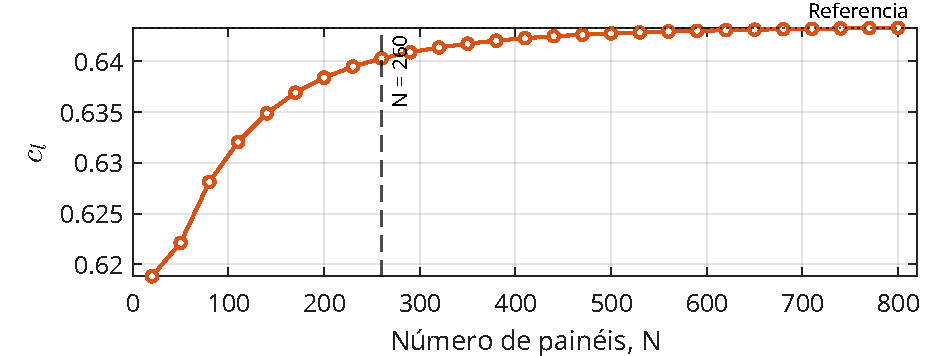
\includegraphics[width=\linewidth]
        {../Comparison/figures/panel_convergence_cl.pdf}
        \caption{Coeficiente de sustentação.}
        \label{fig:convergencia_cl}
    \end{subfigure}
    \hfill
    \begin{subfigure}[t]{0.49\linewidth}
        \centering
        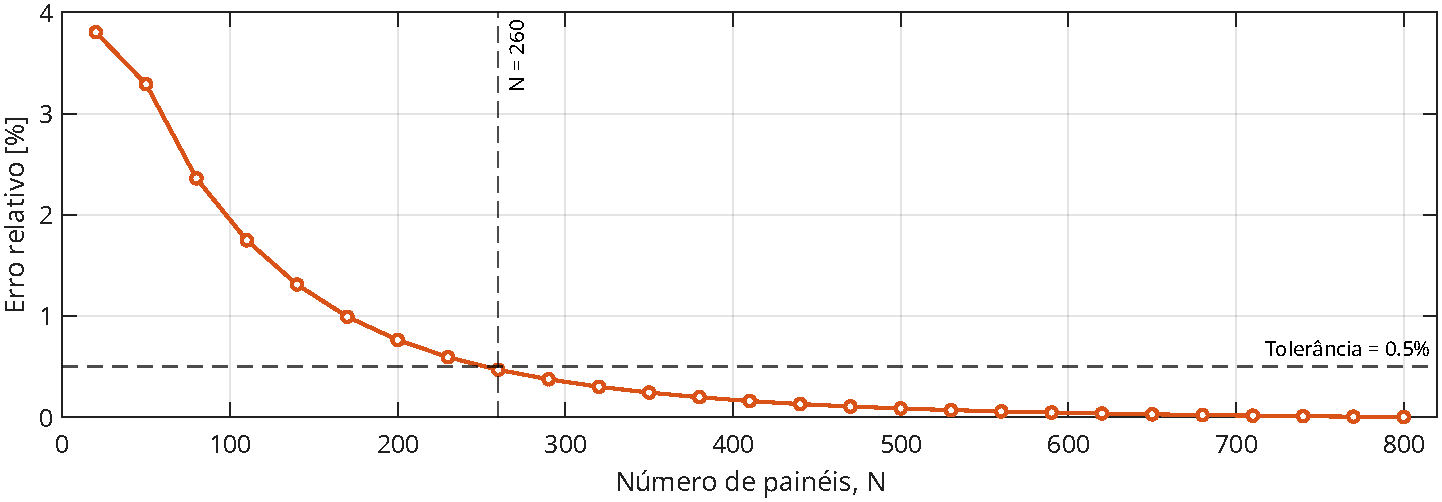
\includegraphics[width=\linewidth]
        {../Comparison/figures/panel_convergence_error.pdf}
        \caption{Erro relativo percentual.}
        \label{fig:convergencia_erro}
    \end{subfigure}

    \caption{Estudo de convergência do método dos
    painéis para $\alpha=5^\circ$.}
    \label{fig:convergencia_paineis}
\end{figure}


A Figura~\ref{fig:painelizacao} mostra a painelização final, com
$N = 260$ painéis e os respetivos pontos de controlo.
\tbd{decidir se se acrescentam os vetores normais e tangentes à figura}
\rasc{Como a interpolação é parametrizada pela distância acumulada ao longo de
cada superfície, com pontos igualmente espaçados nesse parâmetro, os painéis
têm todos aproximadamente o mesmo comprimento. Não há, portanto,
concentração de painéis junto ao bordo de ataque, onde a curvatura da superfície
e os gradientes de velocidade são maiores, nem junto ao bordo de fuga, onde se
impõe a condição de Kutta. Por isso, o bordo de ataque só fica bem descrito
graças ao elevado número de painéis ($N = 260$).}

\begin{figure}[H]
  \centering
  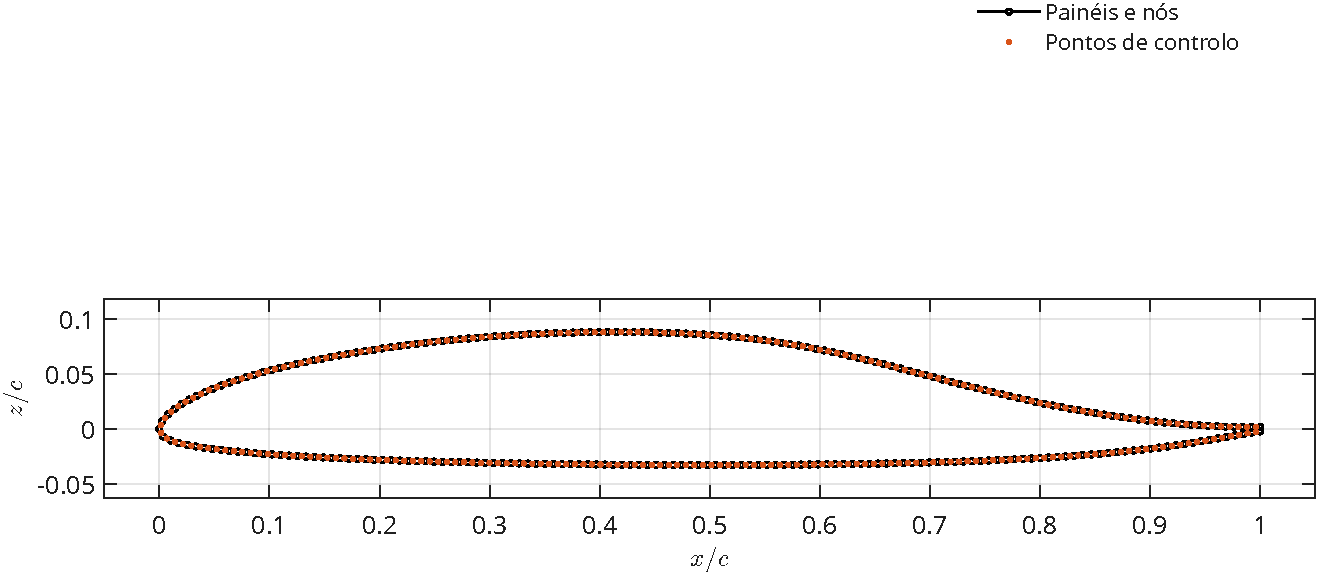
\includegraphics[width=0.8\linewidth]{../Comparison/figures/panelization.pdf}
  \caption{Painelização final do perfil Roncz/Marske-7 com $N=260$ painéis
  e respetivos pontos de controlo.}
  \label{fig:painelizacao}
\end{figure}

% ---------------------------------------------------------------------------
\subsection*{Estudo de convergência da simulação CFD}

{\huge\bfseries\color{red} GONÇALO: ISTO SÃO IDEIAS\par} % REMOVER antes de entregar
% Critério: convergência de malha + independência da solução, justificar a malha.

O estudo de independência de malha foi realizado para quatro configurações
de malha, \rasc{a $\alpha = 5^\circ$} \tbd{confirmar: os $c_l$ ($\approx 0{,}63$) coincidem com o CFD a $5^\circ$}.
A Tabela~\ref{tab:malhas} resume as malhas testadas e a
Figura~\ref{fig:independencia_cfd} apresenta os coeficientes aerodinâmicos e
o indicador de eficiência das malhas.

\begin{table}[H]
  \centering
  \caption{Estudo de independência de malha.}
  \label{tab:malhas}
  \begin{tabular}{lccc}
    \toprule
    Configuração & N.º de células & $c_l$ & Variação de $c_l$ [\%] \\
    \midrule
    0,14 & \tbd{} & \rasc{0,637} & --- \\
    0,10 & \tbd{} & \rasc{0,635} & \rasc{$-0{,}4$} \\
    0,07 & \tbd{} & \rasc{0,618} & \rasc{$-2{,}7$} \\
    0,05 & \tbd{} & \rasc{0,626} & \rasc{$+1{,}4$} \\
    \bottomrule
  \end{tabular}
\end{table}

\begin{figure}[H]
  \centering
  \begin{subfigure}[c]{0.48\linewidth}
    \centering
    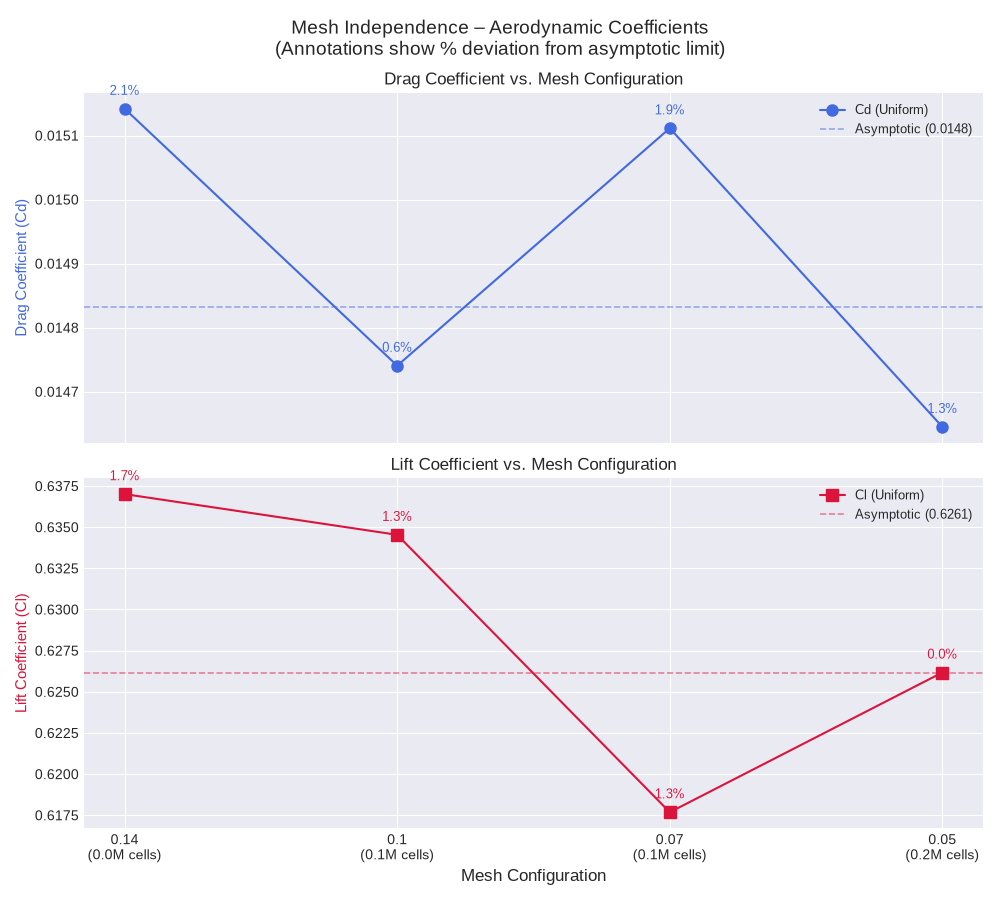
\includegraphics[width=\linewidth]{../CFD/graficos-mesh-independence/Figure_1.png}
    \caption{Coeficientes aerodinâmicos e equilíbrio aerodinâmico.}
  \end{subfigure}\hfill
  \begin{subfigure}[c]{0.48\linewidth}
    \centering
    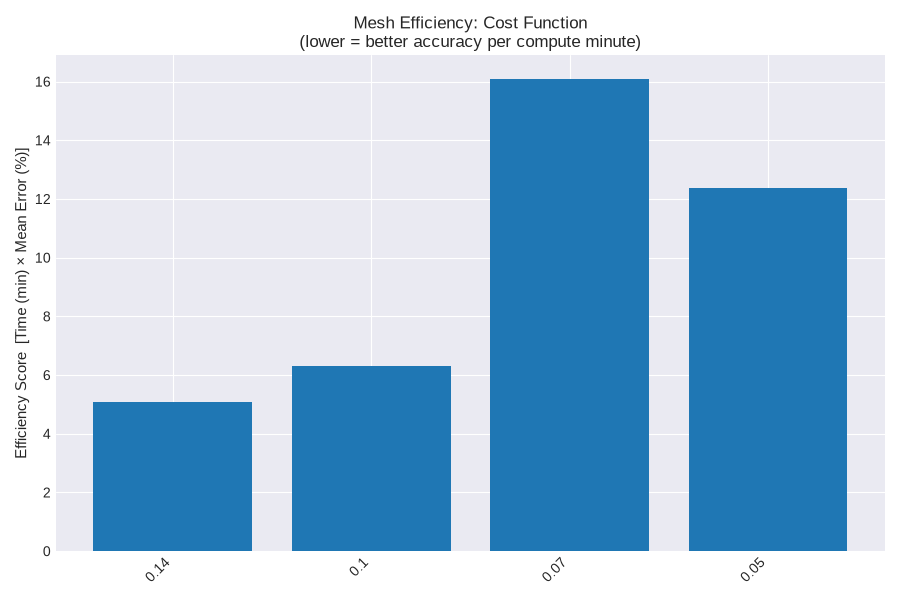
\includegraphics[width=\linewidth]{../CFD/graficos-mesh-independence/Figure_5.png}
    \caption{Indicador de eficiência computacional.}
  \end{subfigure}
  \caption{Estudo de independência da solução CFD e eficiência das malhas.}
  \label{fig:independencia_cfd}
\end{figure}

A Figura~\ref{fig:custo_yplus_cfd} apresenta os tempos de geração da malha
e de simulação, bem como os valores médio, mínimo e máximo de $y^+$ para cada
configuração de malha.

\begin{figure}[H]
  \centering
  \begin{subfigure}[c]{0.48\linewidth}
    \centering
    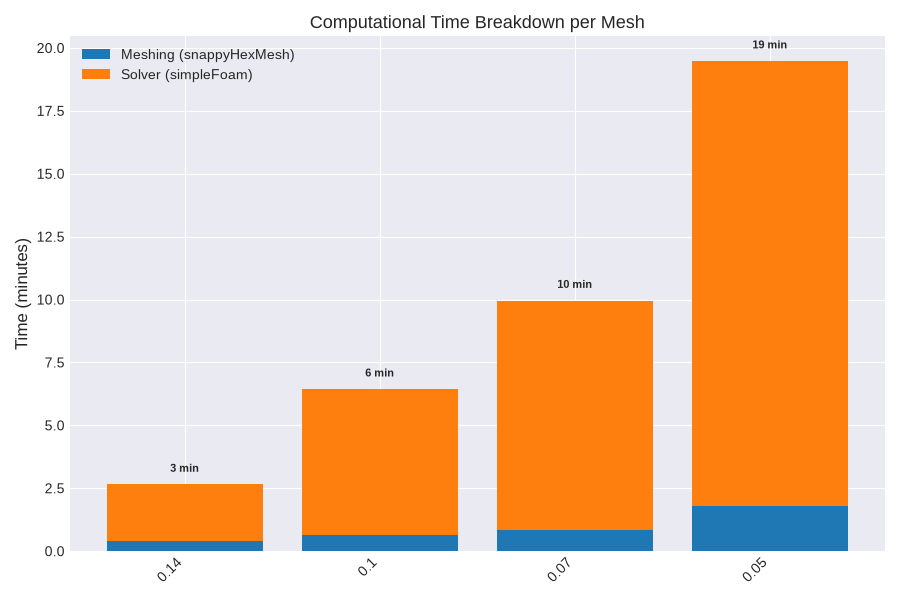
\includegraphics[width=\linewidth]{../CFD/graficos-mesh-independence/Figure_2.png}
    \caption{Tempos de geração de malha e simulação.}
  \end{subfigure}\hfill
  \begin{subfigure}[c]{0.48\linewidth}
    \centering
    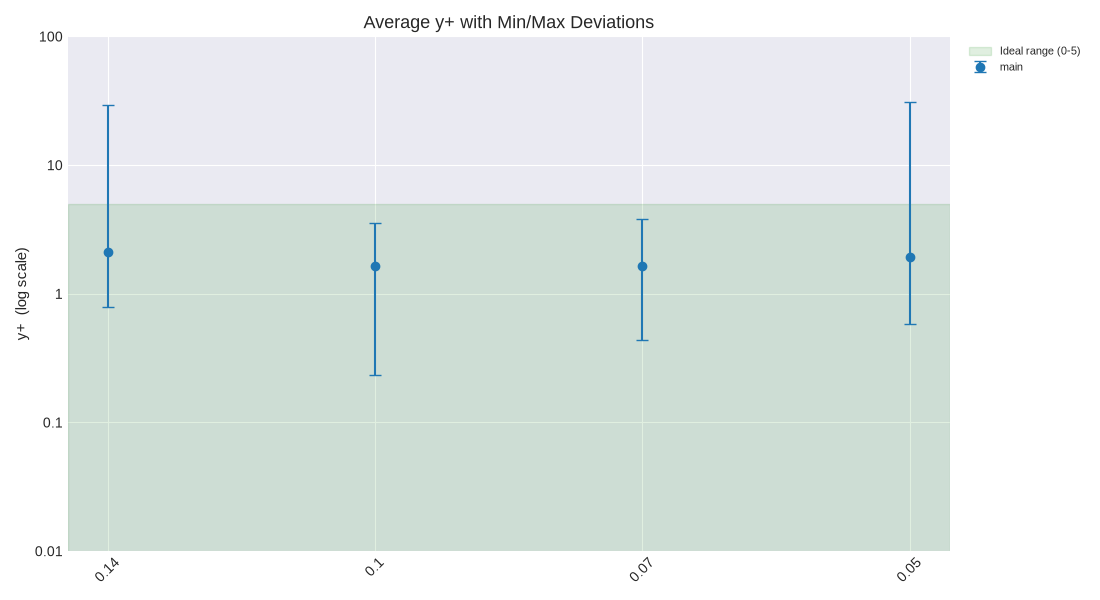
\includegraphics[width=\linewidth]{../CFD/graficos-mesh-independence/Figure_3.png}
    \caption{Estatísticas de $y^+$ por malha.}
  \end{subfigure}
  \caption{Custo computacional e indicadores de resolução junto à parede.}
  \label{fig:custo_yplus_cfd}
\end{figure}

\rasc{O parâmetro de refinamento é o tamanho das células da malha de fundo
(0,14, 0,10, 0,07 e 0,05~m), reduzido aproximadamente por um fator $\sqrt{2}$
entre malhas consecutivas, mantendo-se os níveis de refinamento junto ao
perfil e as camadas prismáticas. Nas quatro malhas, $c_l$ varia entre 0,618 e
0,637, sempre a menos de 2\,\% do valor assintótico (0,626), e $c_d$ entre
0,0146 e 0,0151 (desvios até cerca de 2\,\%). A variação não é monótona, já que $c_l$
desce até à malha 0,07 e volta a subir na malha 0,05, o que indica que as
diferenças restantes são da ordem do erro numérico e iterativo, e não uma
tendência sistemática de refinamento.

O custo, por outro lado, cresce rapidamente. O tempo total, somando a geração
da malha e a simulação, passa de cerca de 3~min (0,14) para 6~min (0,10), 10~min (0,07) e
19~min (0,05). O $y^+$ médio está entre 1,6 e 2,1 em todas as malhas, dentro
do intervalo pretendido ($y^+ < 5$), mas as malhas 0,14 e 0,05 apresentam
máximos locais próximos de 30, enquanto nas malhas 0,10 e 0,07 o máximo é
inferior a 4.

Pelo indicador de eficiência (Figura~\ref{fig:independencia_cfd}b), a malha
0,14 é a de menor custo para a precisão obtida, seguida da 0,10. Escolheu-se a
malha 0,10, que tem um custo apenas ligeiramente superior, $c_l$ a 1,3\,\% do
valor assintótico e $y^+ < 5$ em todo o perfil, garantindo a resolução da
subcamada viscosa. \tbd{confirmar com o Gonçalo a malha usada nas simulações
finais e o n.º de células de cada malha}}

A Figura~\ref{fig:qualidade_malha} apresenta os indicadores de qualidade de
cada configuração de malha, obtidos com o \texttt{checkMesh}, nomeadamente a
não-ortogonalidade máxima e média, a \emph{skewness} máxima, a razão de aspeto
máxima e o número de células problemáticas.

\begin{figure}[H]
  \centering
  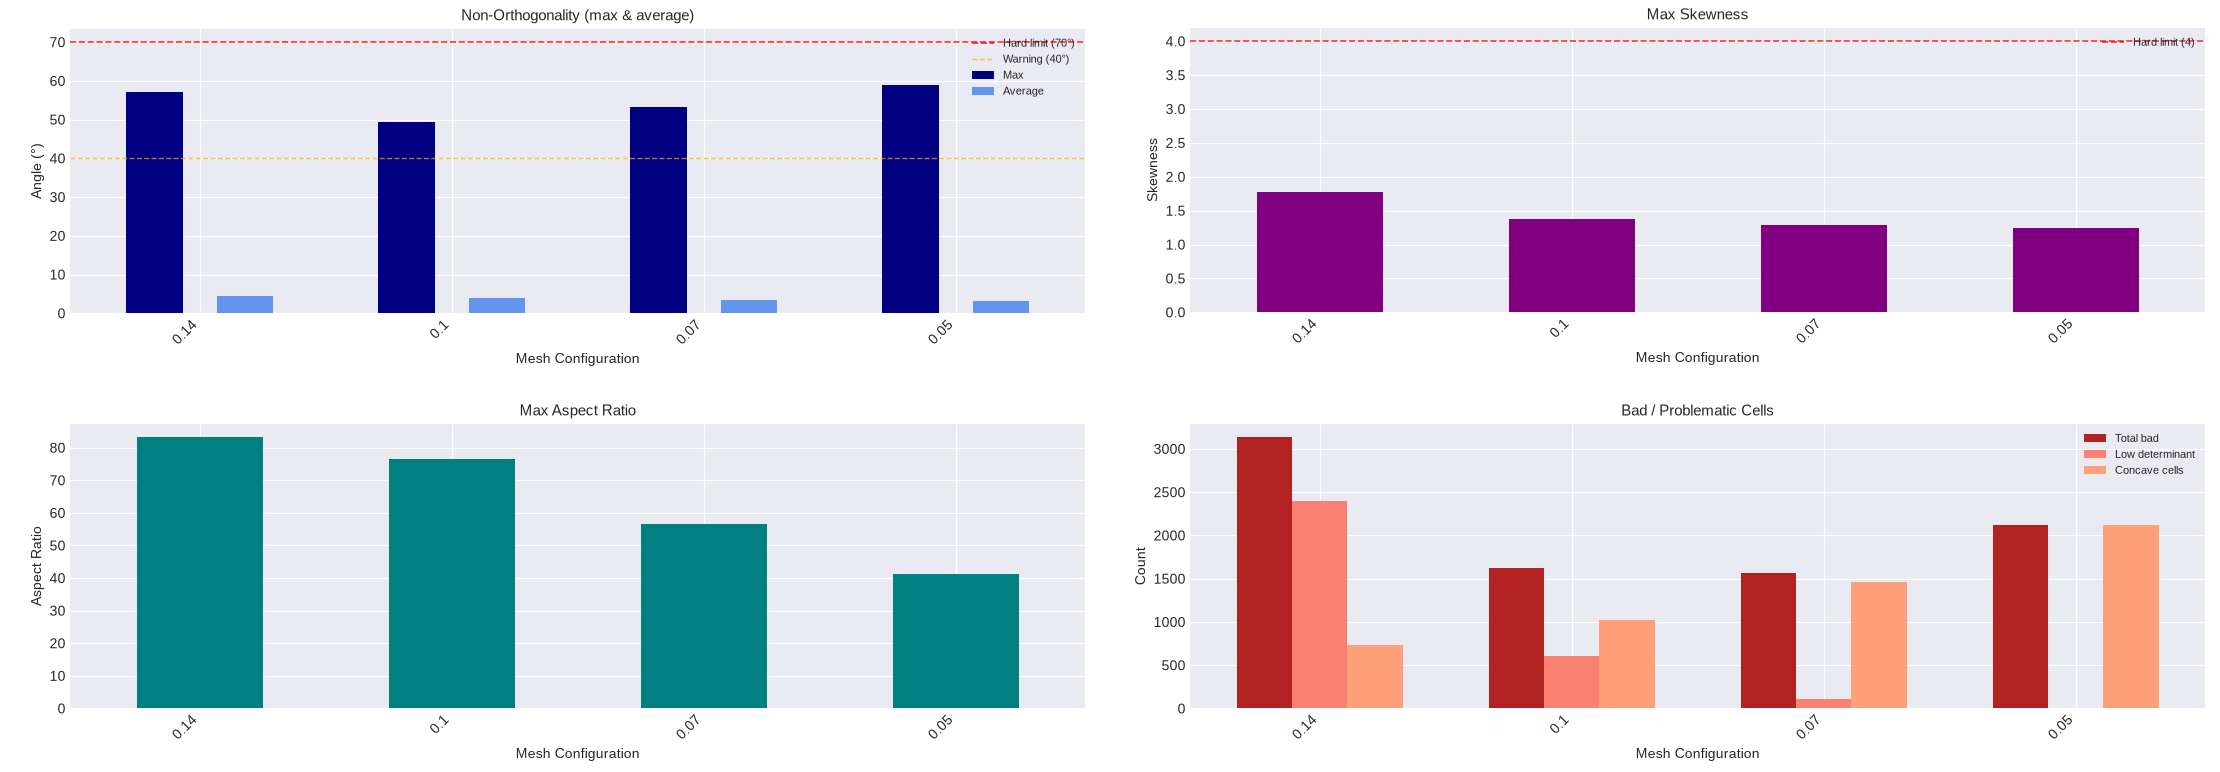
\includegraphics[width=\linewidth]{../CFD/graficos-mesh-independence/Figure_4_2x2.png}
  \caption{Indicadores de qualidade das malhas (\texttt{checkMesh}).}
  \label{fig:qualidade_malha}
\end{figure}

% ---------------------------------------------------------------------------
\subsection*{Comparação de métodos}

\paragraph{Coeficiente de sustentação.}
A Figura~\ref{fig:cl_alpha} sobrepõe os $c_l$ previstos pelos três métodos,
calculados de $-20^\circ$ a $20^\circ$ com passo de $0{,}5^\circ$ nos perfis
delgados, de $-20^\circ$ a $20^\circ$ com passo de $5^\circ$ nos painéis e de
$0^\circ$ a $20^\circ$ com passo de $5^\circ$ no CFD. A Tabela~\ref{tab:cl} dá os valores nos
ângulos comuns.

\begin{figure}[H]
  \centering
  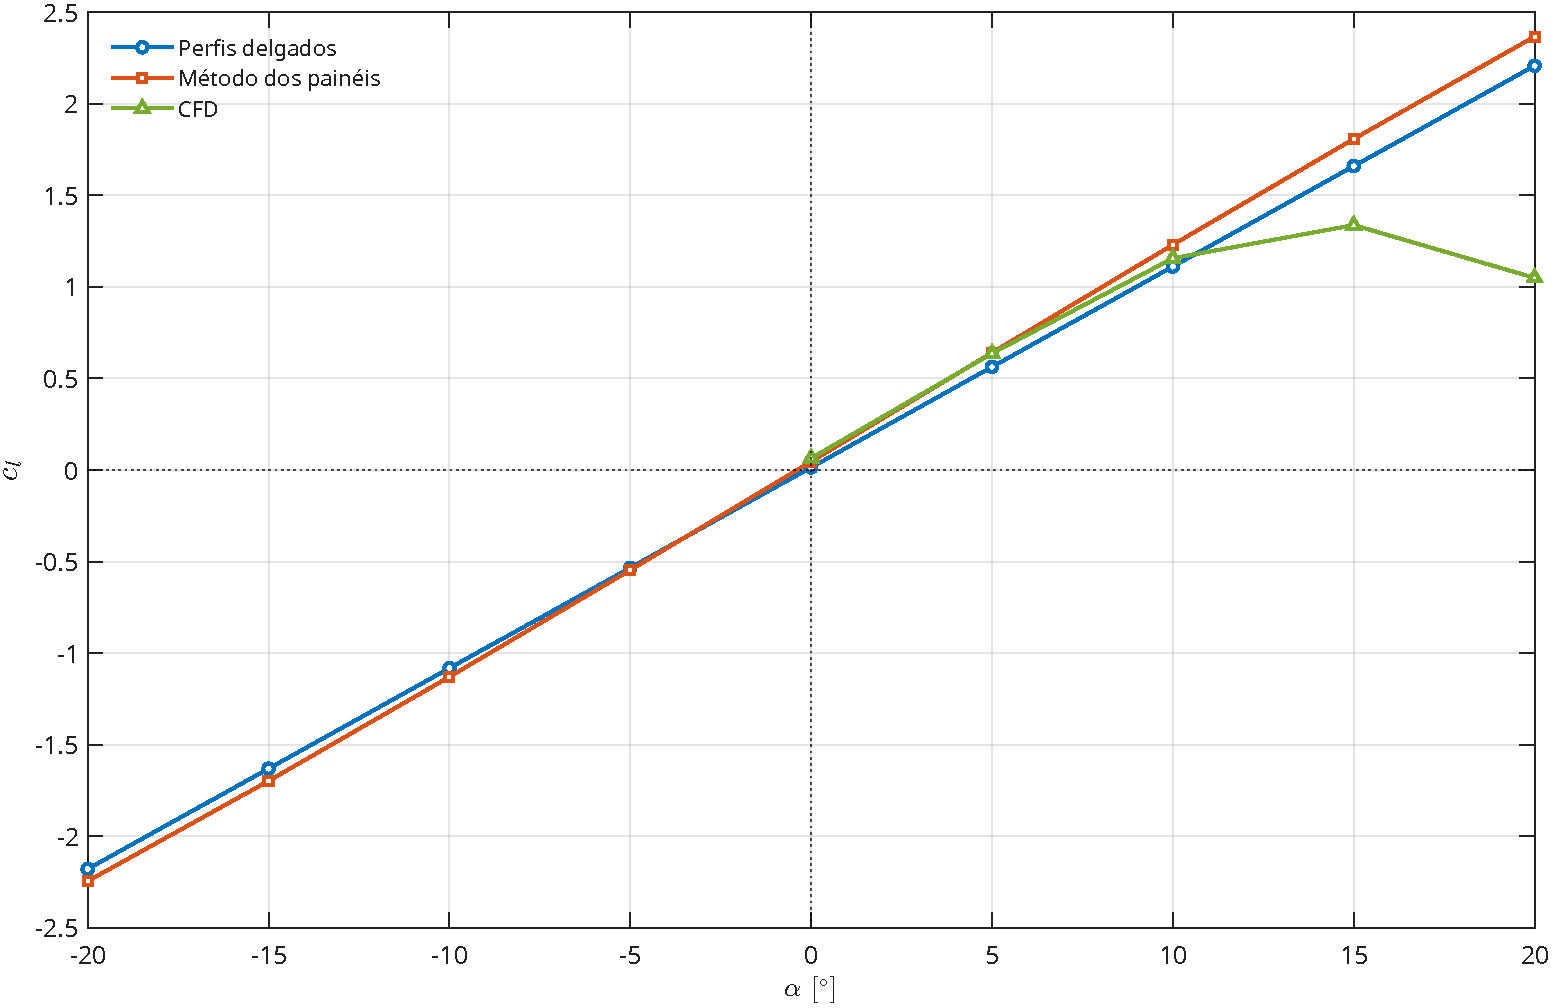
\includegraphics[width=0.7\linewidth]{../Comparison/figures/lift_comparison.pdf}
  \caption{Coeficiente de sustentação em função do ângulo de ataque pelos três
  métodos.}
  \label{fig:cl_alpha}
\end{figure}

\begin{table}[H]
  \centering
  \caption{Coeficiente de sustentação previsto por cada método.}
  \label{tab:cl}
  \begin{tabular}{lccccc}
    \toprule
    Método & $0^\circ$ & $5^\circ$ & $10^\circ$ & $15^\circ$ & $20^\circ$ \\
    \midrule
    Perfis delgados & 0,01 & 0,56 & 1,11 & 1,66 & 2,21 \\
    Painéis         & 0,05 & 0,64 & 1,23 & 1,81 & 2,37 \\
    CFD             & 0,06 & 0,64 & 1,16 & 1,34 & 1,05 \\
    \bottomrule
  \end{tabular}
\end{table}

Na zona linear ($0^\circ$ a $10^\circ$) os três métodos concordam
qualitativamente, mas denota-se que o método dos painéis prevê sistematicamente mais
sustentação do que a teoria dos perfis delgados ($+0{,}08$ a $5^\circ$, $+0{,}12$
a $10^\circ$). A diferença entre eles devem-se aos fenómenos físicos considerados em cada método, e às simplificacões enraizadas nos mesmos. O método dos painéis e o método dos perfis delgados não consideram viscosidade. A teoria dos perfis delgados
representa o perfil apenas pela linha média, ignorando a espessura do perfil, enquanto o método dos painéis
discretiza o contorno real, com 12\,\% de espessura, no qual o escoamento acelera
no extradorso, aumentando assim o declive da curva de sustentação.

O CFD acompanha o método dos painéis até $5^\circ$, mas a diferença entre
os dois cresce rapidamente com o ângulo de ataque. É praticamente nula até
$5^\circ$ e passa para $0{,}07$ a $10^\circ$, $0{,}47$ a $15^\circ$ e $1{,}32$ a
$20^\circ$. Esta diferença deve-se ao facto de a análise de CFD considerar o
efeito da viscosidade. Com o aumento do ângulo de ataque, o gradiente adverso
de pressão no extradorso aumenta e a camada limite torna-se mais espessa, o que
altera a forma efetiva do perfil junto ao bordo de fuga e reduz a circulação.
Daí a diferença de $0{,}07$ a $10^\circ$. Acima de $10^\circ$ o CFD deixa de ter
comportamento linear, porque o gradiente adverso de pressão passa a ser
suficiente para provocar o descolamento ou separação da camada limite. A
$15^\circ$ o descolamento começa junto ao bordo de fuga
\tbd{$x/c$ onde a tensão de corte no extradorso se anula, pedir ao Gonçalo} e o
$c_l$ fica-se por $1{,}34$. A $20^\circ$ o descolamento começa logo junto ao
bordo de ataque e ocupa quase todo o extradorso (Figura~\ref{fig:linhas}), pelo
que o $c_l$ desce para $1{,}05$ e o arrasto sobe para $c_d = 0{,}27$, quase todo
de pressão. O perfil entra, portanto, em perda entre $15^\circ$ e $20^\circ$.
\tbd{confirmar se a simulação a $20^\circ$ convergiu ou se o escoamento é não
estacionário}

Os dois métodos potenciais continuam lineares até $20^\circ$ porque assumem
que o escoamento está sempre colado. Como não modelam a camada limite, não há
nada que possa descolar, e a condição de Kutta obriga o escoamento a sair
suavemente pelo bordo de fuga independentemente do ângulo de ataque. Assim, não
conseguem prever a perda nem o $c_{l,\max}$.

\paragraph{Ângulo de sustentação nula e declive.}
A Tabela~\ref{tab:alpha0} apresenta o ângulo de sustentação nula e o declive da
curva $c_l(\alpha)$ na zona linear, obtidos por regressão linear entre
\rasc{$0^\circ$ e $10^\circ$. Esta gama corresponde à zona em que o declive
local da curva $c_l(\alpha)$ do CFD, calculado entre ângulos consecutivos,
difere menos de 10\,\% do declive entre $0^\circ$ e $5^\circ$; como os métodos
potenciais são lineares em toda a gama, é o CFD que a limita.}

\begin{table}[H]
  \centering
  \caption{Ângulo de sustentação nula e declive da curva de sustentação na zona
  linear.}
  \label{tab:alpha0}
  \begin{tabular}{lcc}
    \toprule
    Método & $\alpha_{L=0}$ [$^\circ$] & $dc_l/d\alpha$ [rad$^{-1}$] \\
    \midrule
    Perfis delgados & $-0{,}13$ & 6,28 \\
    Painéis         & $-0{,}39$ & 6,78 \\
    CFD             & $-0{,}67$ & 6,26 \\
    \bottomrule
  \end{tabular}
\end{table}

\rasc{Apesar de o perfil ter 2,8\,\% de curvatura, $\alpha_{L=0}$ é muito
pequeno nos três métodos (entre $-0{,}13^\circ$ e $-0{,}67^\circ$). Na teoria dos
perfis delgados,
\[
  \alpha_{L=0} = \frac{1}{\pi}\int_0^{\pi}\frac{dz_c}{dx}\,(1-\cos\theta)\,d\theta ,
\]
em que o peso $(1-\cos\theta)$ é máximo junto ao bordo de fuga
($\theta \to \pi$). O \emph{reflex} da linha média nessa zona (mínimo de
$-0{,}5\,\%$ em $x/c = 0{,}90$) dá declives positivos com o maior peso, que
compensam quase totalmente a contribuição da curvatura da parte dianteira. As
diferenças entre métodos (cerca de $0{,}5^\circ$) correspondem a
$\Delta c_l \approx 0{,}05$, a mesma ordem de grandeza dos próprios $c_l$ a
$0^\circ$, pelo que $\alpha_{L=0}$ é muito sensível a pequenas diferenças de
modelação. No CFD, $\alpha_{L=0}$ é extrapolado da reta ajustada entre $0^\circ$
e $10^\circ$, uma vez que não foram simulados ângulos negativos.

O declive da teoria dos perfis delgados é exatamente $2\pi$, independente da
geometria. O método dos painéis dá mais 8\,\% (6,78~rad$^{-1}$), o que está de
acordo com a correção clássica para a espessura,
$c_{l\alpha} \approx 2\pi\,(1 + 0{,}77\,t/c) \approx 6{,}87$~rad$^{-1}$ para
$t/c = 0{,}121$. O CFD dá praticamente $2\pi$ (6,26~rad$^{-1}$), porque o aumento devido
à espessura é compensado pela redução viscosa da circulação. O declive real
fica assim cerca de 8\,\% abaixo do previsto pelo método dos painéis.}

\paragraph{Tempo de cálculo e recursos.}
A Tabela~\ref{tab:custo} compara o custo de cada método, num computador com
\tbd{CPU, RAM}.

\begin{table}[H]
  \centering
  \caption{Custo computacional de cada método.}
  \label{tab:custo}
  \begin{tabular}{lccc}
    \toprule
    Método & Software & N.º de ângulos & Tempo de cálculo \\
    \midrule
    Perfis delgados & MATLAB   & 81 & $\approx 0{,}1$~ms (total) \\
    Painéis         & MATLAB   & 9  & $\approx 1{,}5$~s (total) \\
    CFD             & OpenFOAM & 5  & \rasc{$\approx 6$~min} por ângulo \tbd{confirmar} \\
    \bottomrule
  \end{tabular}
\end{table}

\rasc{A diferença de custo é ainda maior quando se inclui a preparação. Nos
métodos potenciais, basta um \emph{script} que lê as coordenadas do perfil,
e mudar de perfil ou de ângulo de ataque é imediato. No CFD é preciso construir
o domínio, gerar e verificar a malha (incluindo as camadas prismáticas para
$y^+ \approx 1$), definir as condições de fronteira e o modelo de turbulência,
fazer o estudo de independência de malha e acompanhar a convergência de cada
simulação. Além disso, como se rodou o perfil, a malha tem de ser gerada de
novo para cada ângulo. Esta preparação demora horas a dias, contra minutos nos
métodos potenciais.}

\paragraph{Vantagens, desvantagens e gama de aplicação.}
\rasc{A teoria dos perfis delgados é analítica, quase não tem custo e mostra
diretamente o efeito da curvatura através de $\alpha_{L=0}$. Em contrapartida,
ignora a espessura e a viscosidade, tem uma singularidade no bordo de ataque,
onde a velocidade tende para infinito, e dá sempre o mesmo declive de $2\pi$,
sem prever arrasto nem perda. Serve para estimativas iniciais de $c_l$ e de
$\alpha_{L=0}$ na zona linear, entre $0^\circ$ e cerca de $10^\circ$.

O método dos painéis usa a geometria real e, com um custo de segundos, dá
também a distribuição de $C_p$, as linhas de corrente e o ponto de estagnação,
o que o torna útil para comparar perfis rapidamente. Como não tem viscosidade,
não prevê o arrasto nem a perda, sobrestima $c_l$ e o pico de sucção a ângulos
elevados, e o resultado depende do número de painéis. Deve usar-se com o
escoamento colado, até cerca de $10^\circ$.

O CFD é o único dos três que inclui a viscosidade e a turbulência, e por isso o
único que prevê o arrasto, o descolamento e a perda. O preço é um custo de
preparação e de cálculo muito maior, resultados que dependem da malha e do
modelo de turbulência e uma convergência difícil depois da perda. É
indispensável perto e depois da perda, acima de cerca de $10^\circ$, e para
calcular o arrasto.}

\paragraph{Linhas de corrente.}
A Figura~\ref{fig:linhas} apresenta as linhas de corrente previstas pelo método
dos painéis e pela simulação CFD para $\alpha = 0^\circ$, $5^\circ$ e
$20^\circ$.

\begin{figure}[H]
  \centering
  \begin{subfigure}[c]{0.48\linewidth}
    \centering
    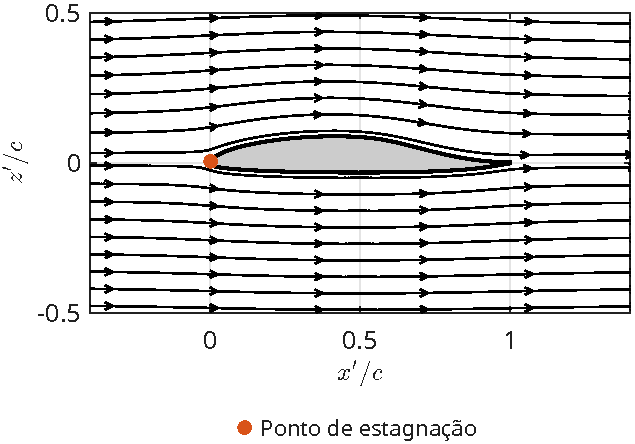
\includegraphics[width=\linewidth]{../Comparison/figures/panel_streamlines_00.pdf}
    \caption{Painéis, $\alpha=0^\circ$.}
  \end{subfigure}\hfill
  \begin{subfigure}[c]{0.48\linewidth}
    \centering
    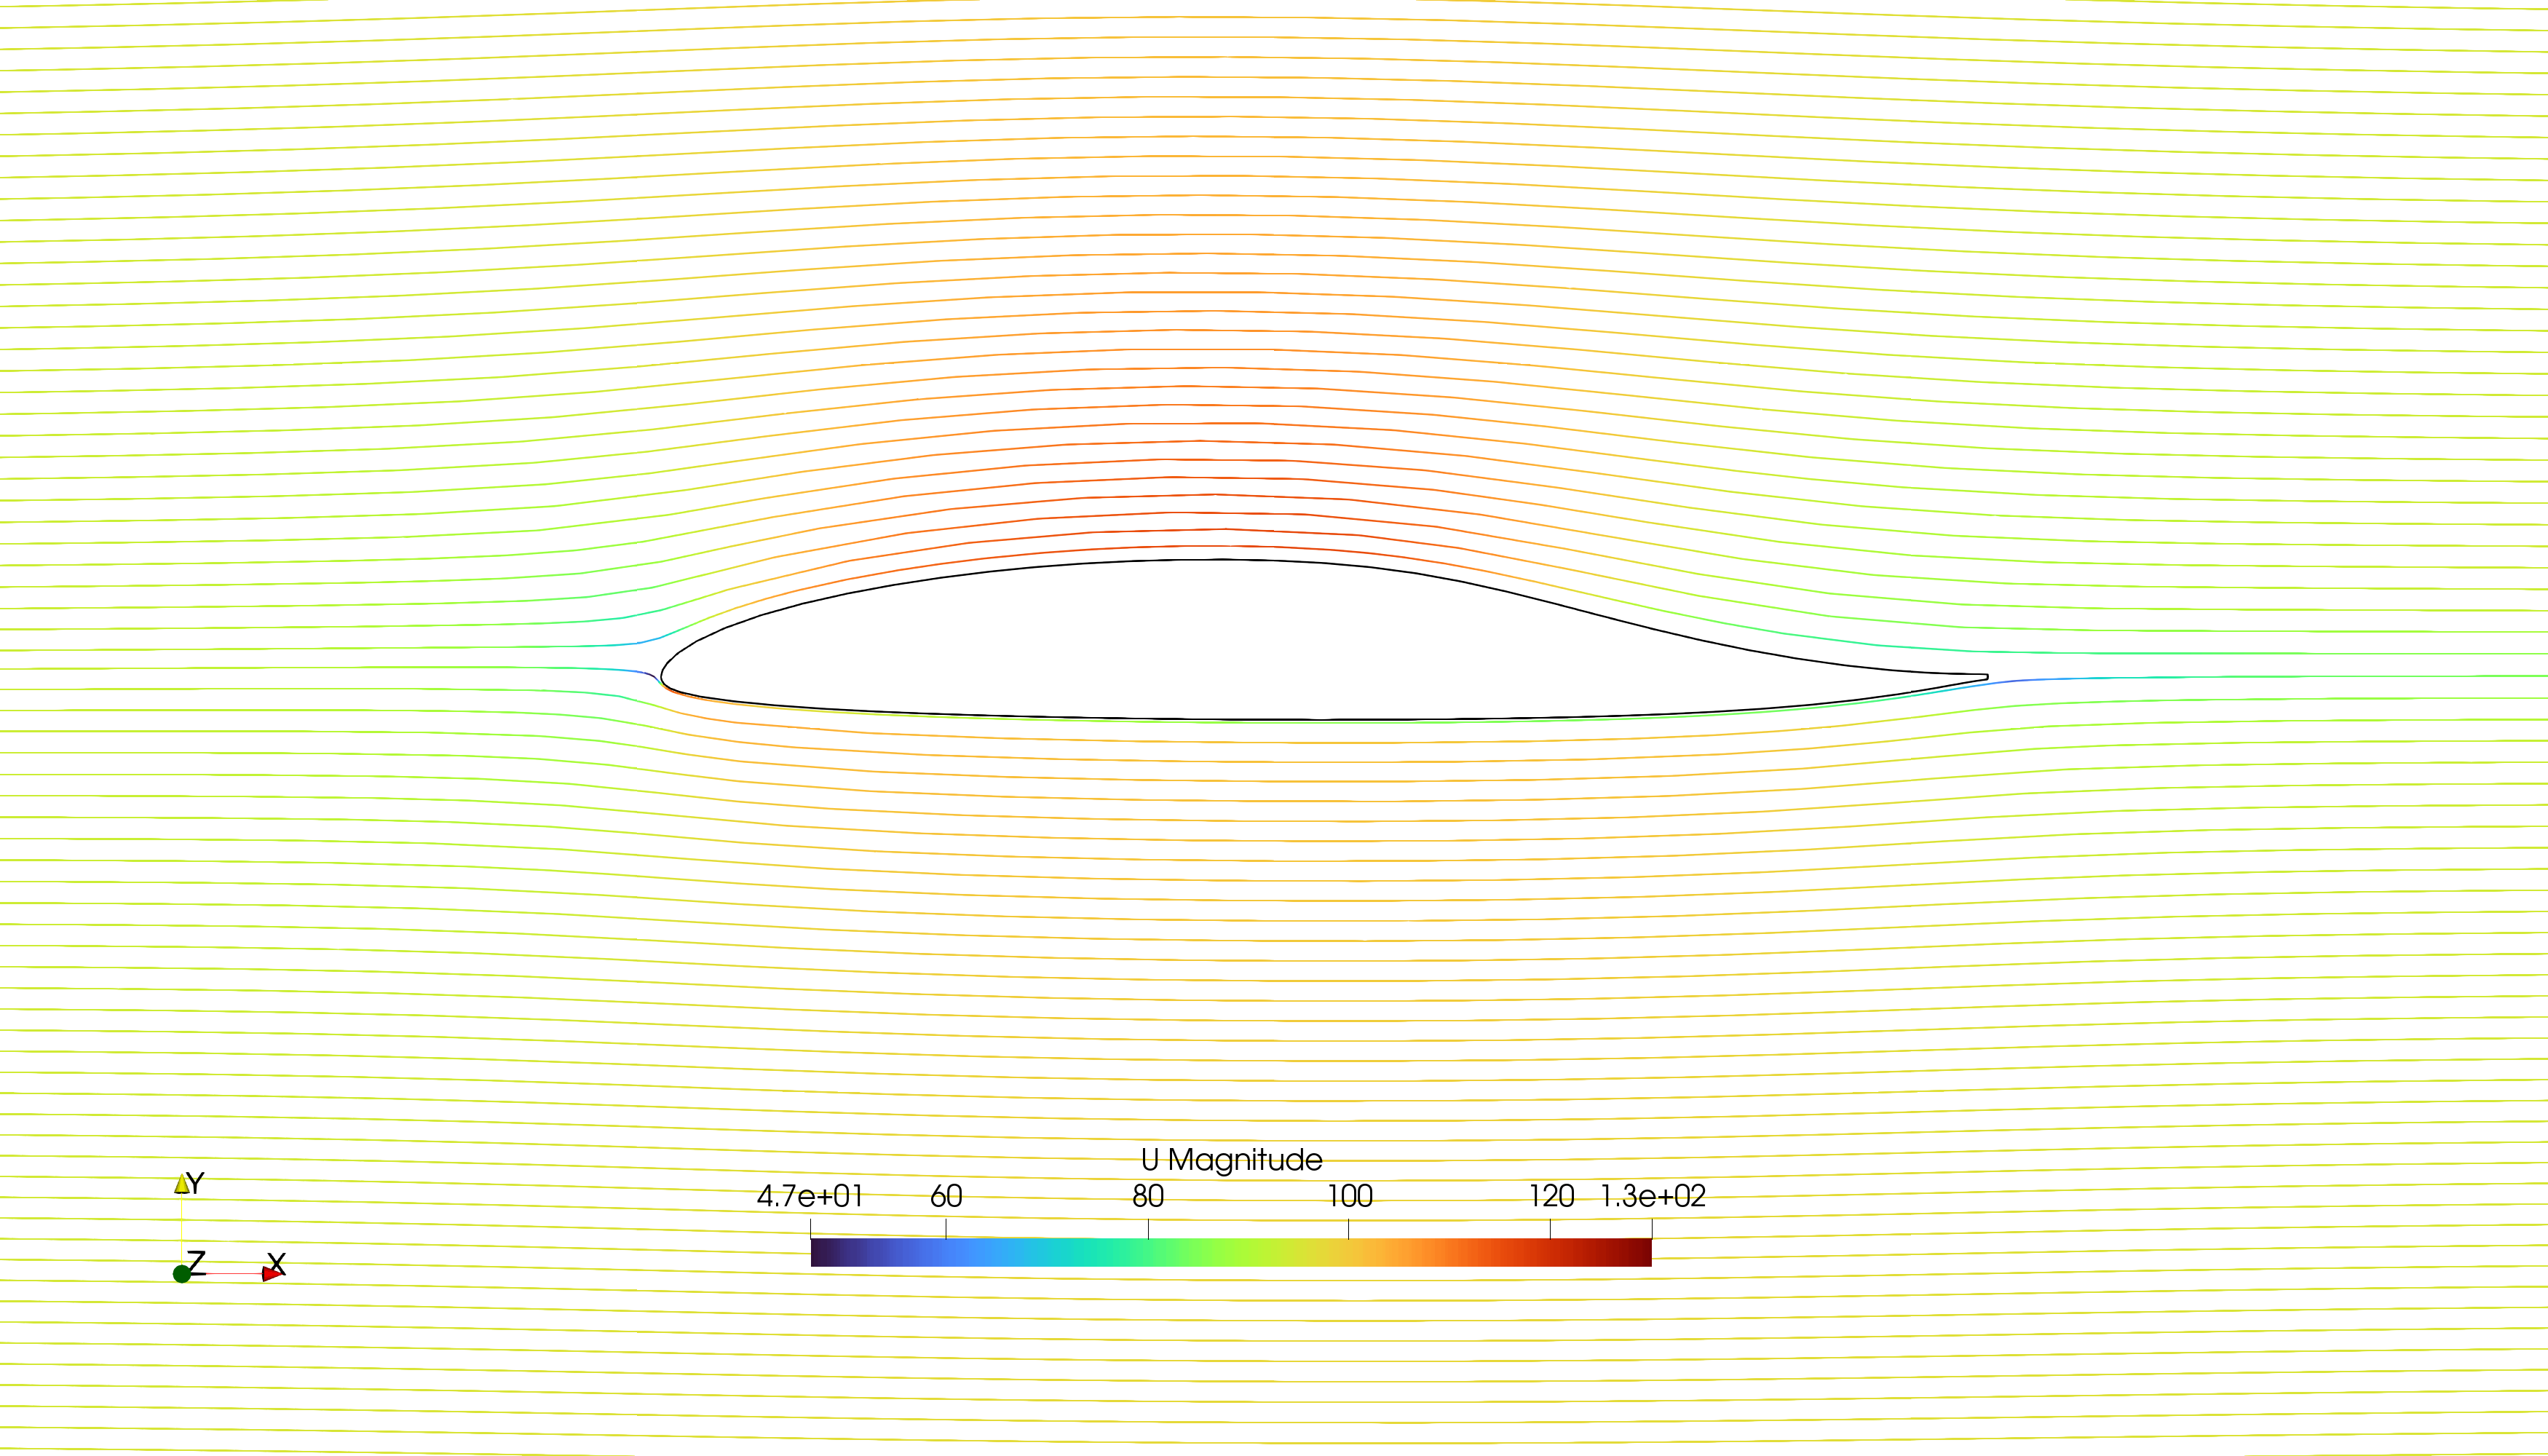
\includegraphics[width=\linewidth]{../CFD/Streamlines/0deg.png}
    \caption{CFD, $\alpha=0^\circ$.}
  \end{subfigure}
  \par\smallskip
  \begin{subfigure}[c]{0.48\linewidth}
    \centering
    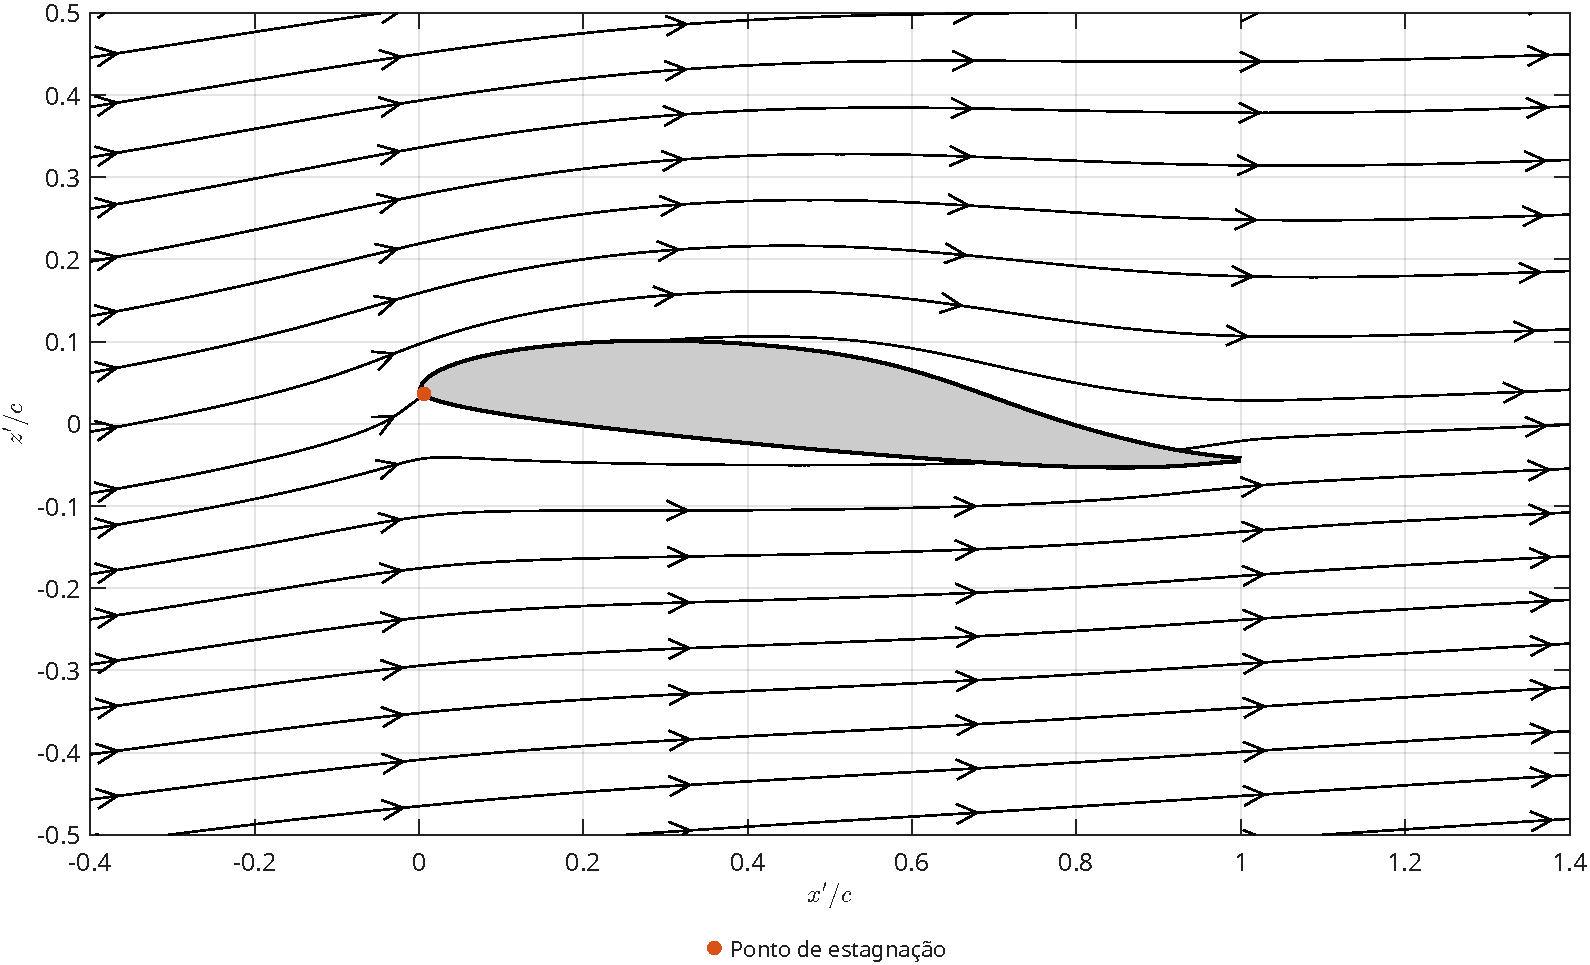
\includegraphics[width=\linewidth]{../Comparison/figures/panel_streamlines_05.pdf}
    \caption{Painéis, $\alpha=5^\circ$.}
  \end{subfigure}\hfill
  \begin{subfigure}[c]{0.48\linewidth}
    \centering
    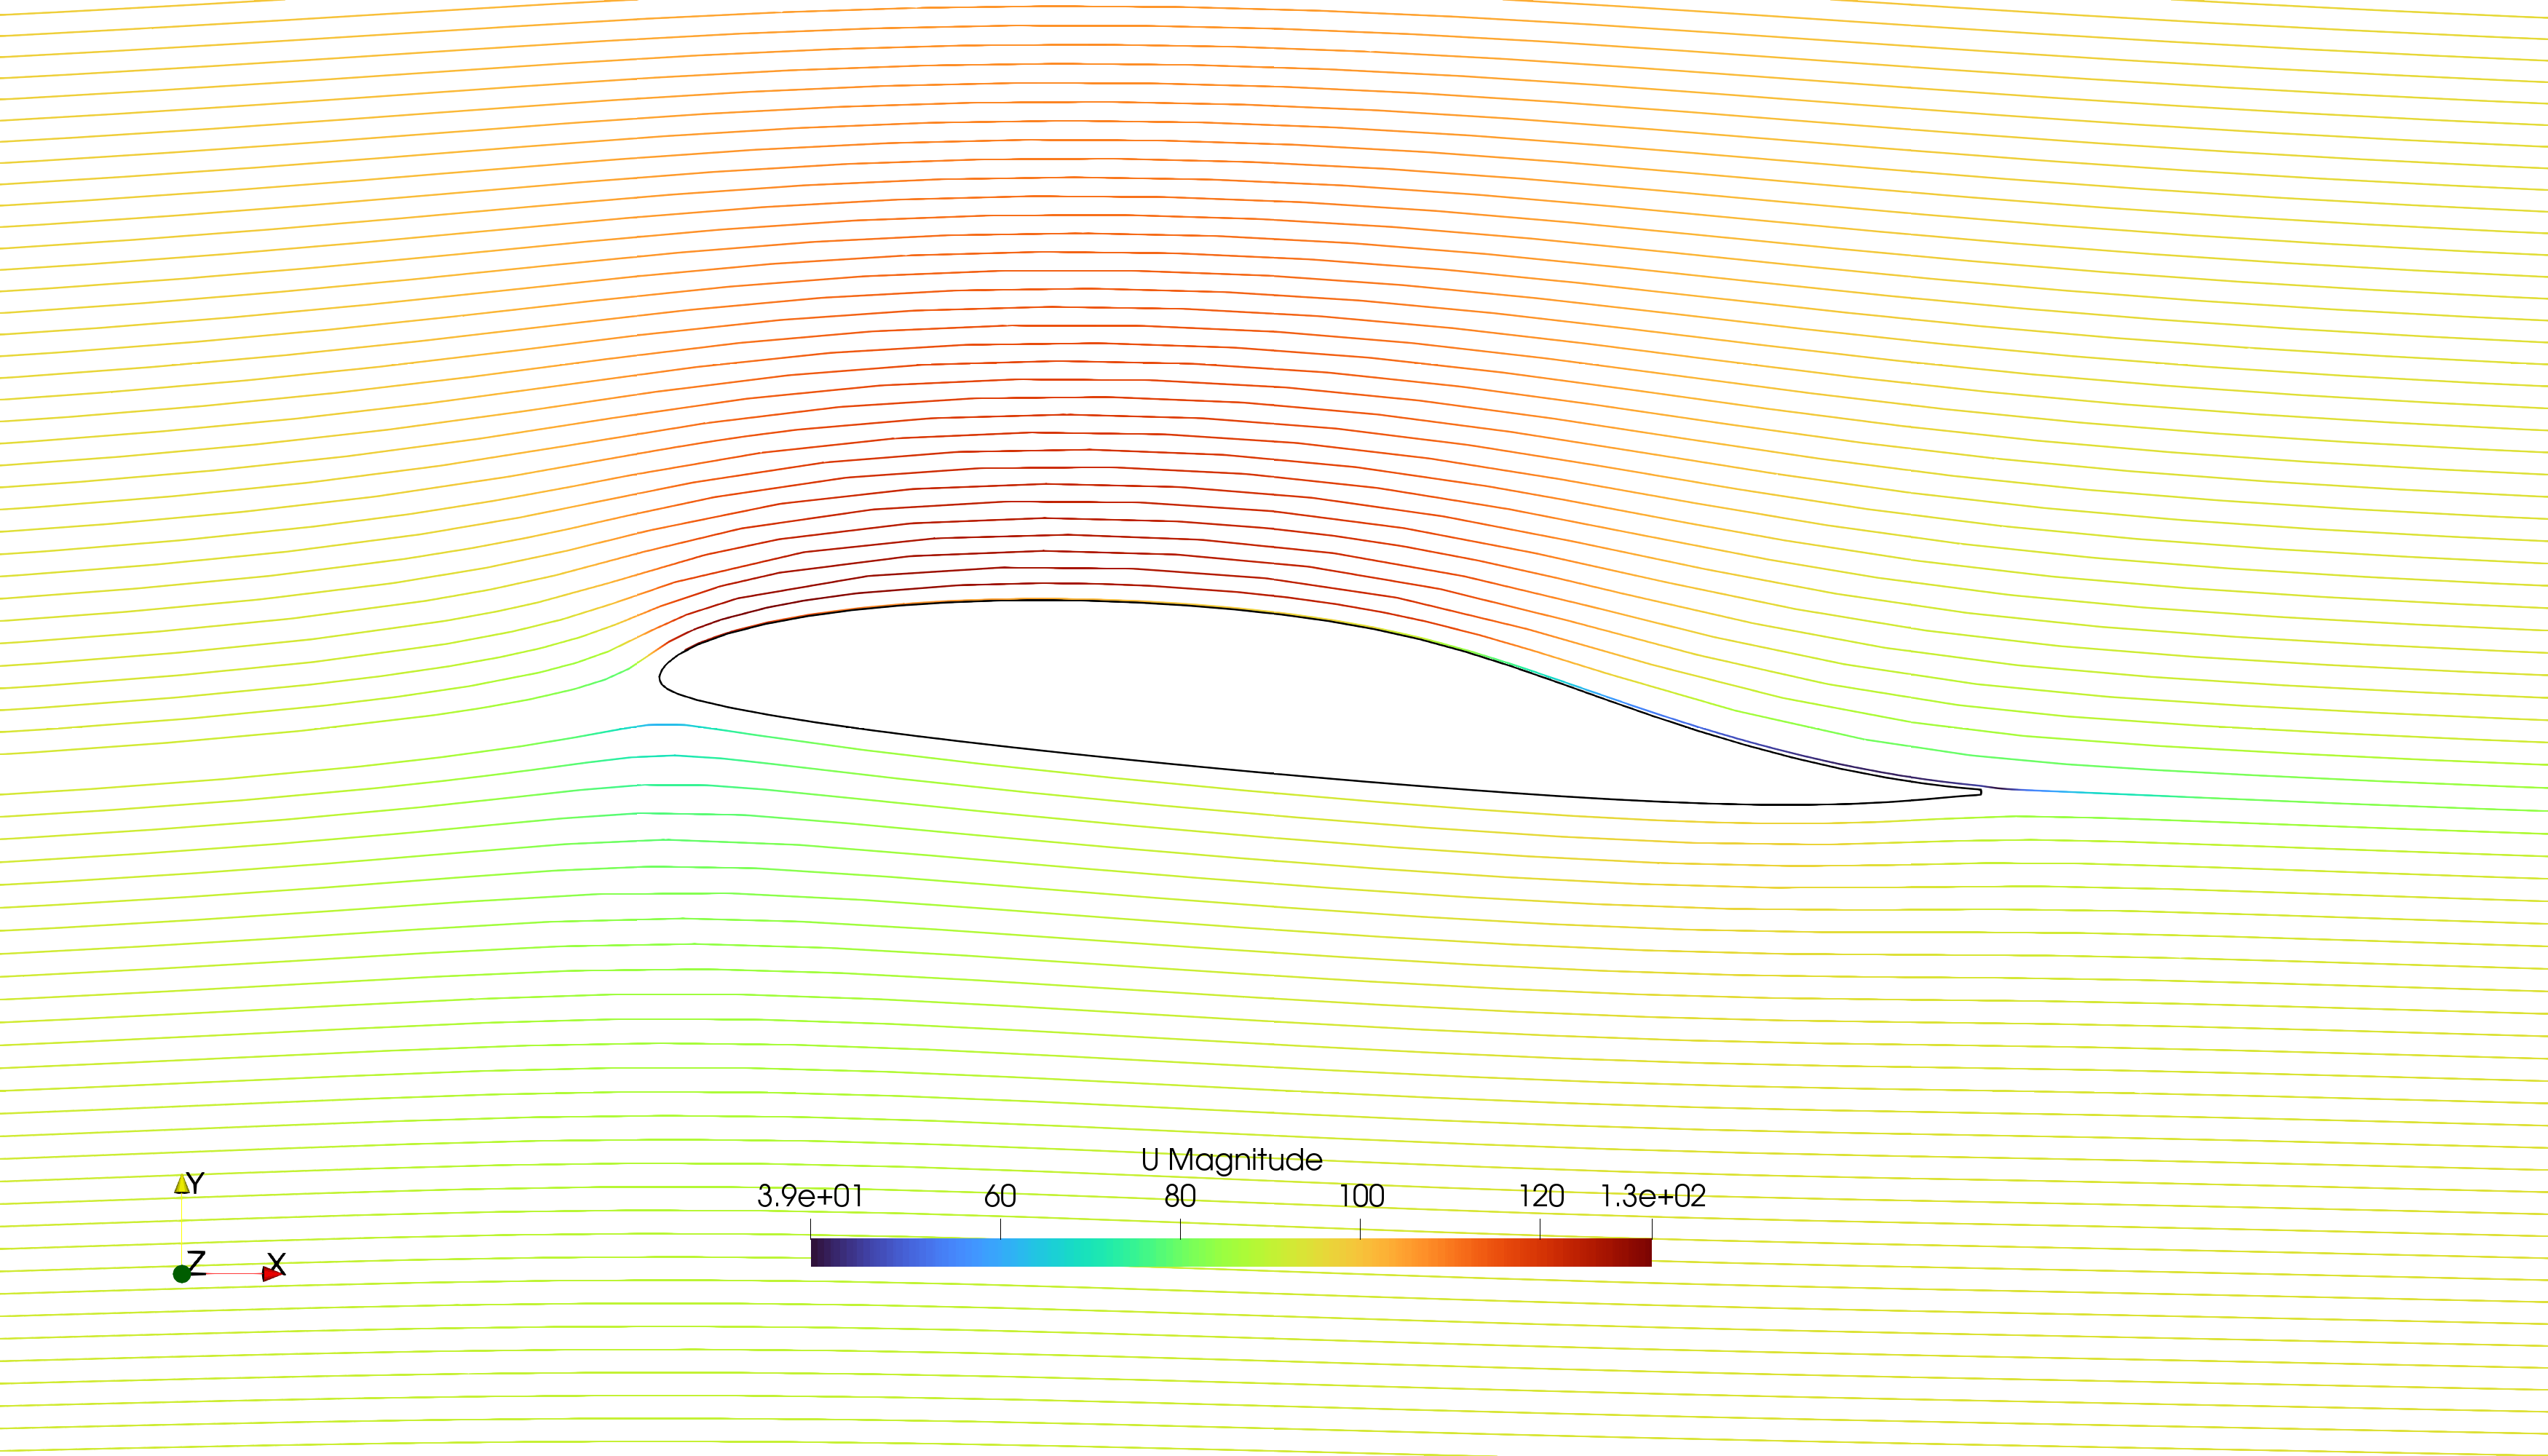
\includegraphics[width=\linewidth]{../CFD/Streamlines/5deg.png}
    \caption{CFD, $\alpha=5^\circ$.}
  \end{subfigure}
  \par\smallskip
  \begin{subfigure}[c]{0.48\linewidth}
    \centering
    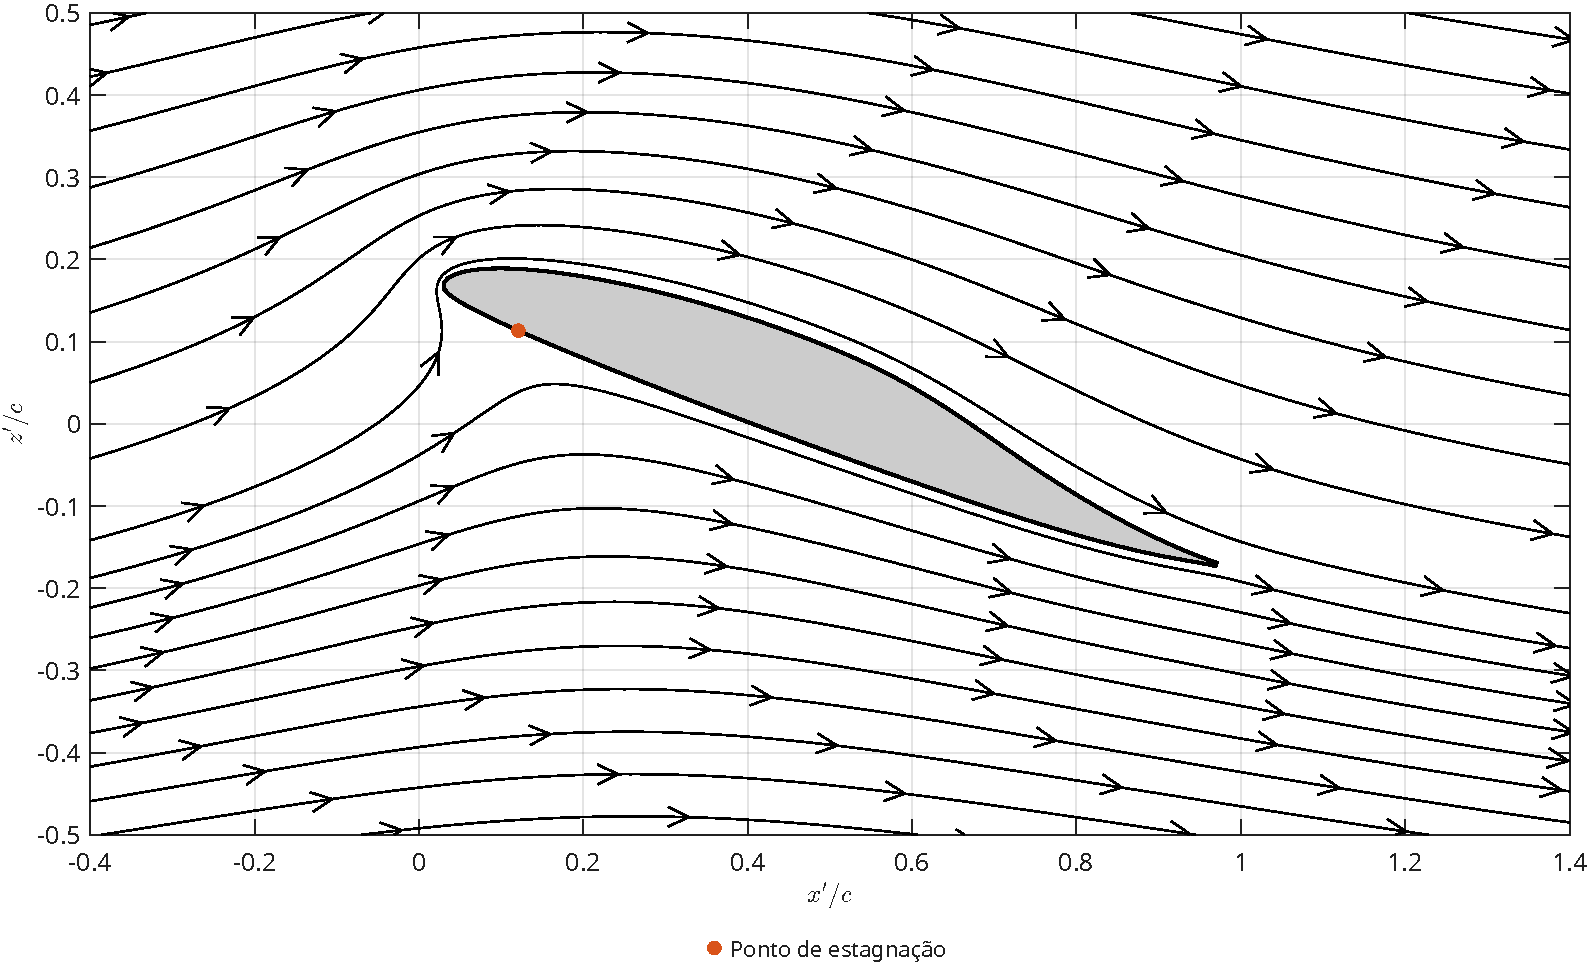
\includegraphics[width=\linewidth]{../Comparison/figures/panel_streamlines_20.pdf}
    \caption{Painéis, $\alpha=20^\circ$.}
  \end{subfigure}\hfill
  \begin{subfigure}[c]{0.48\linewidth}
    \centering
    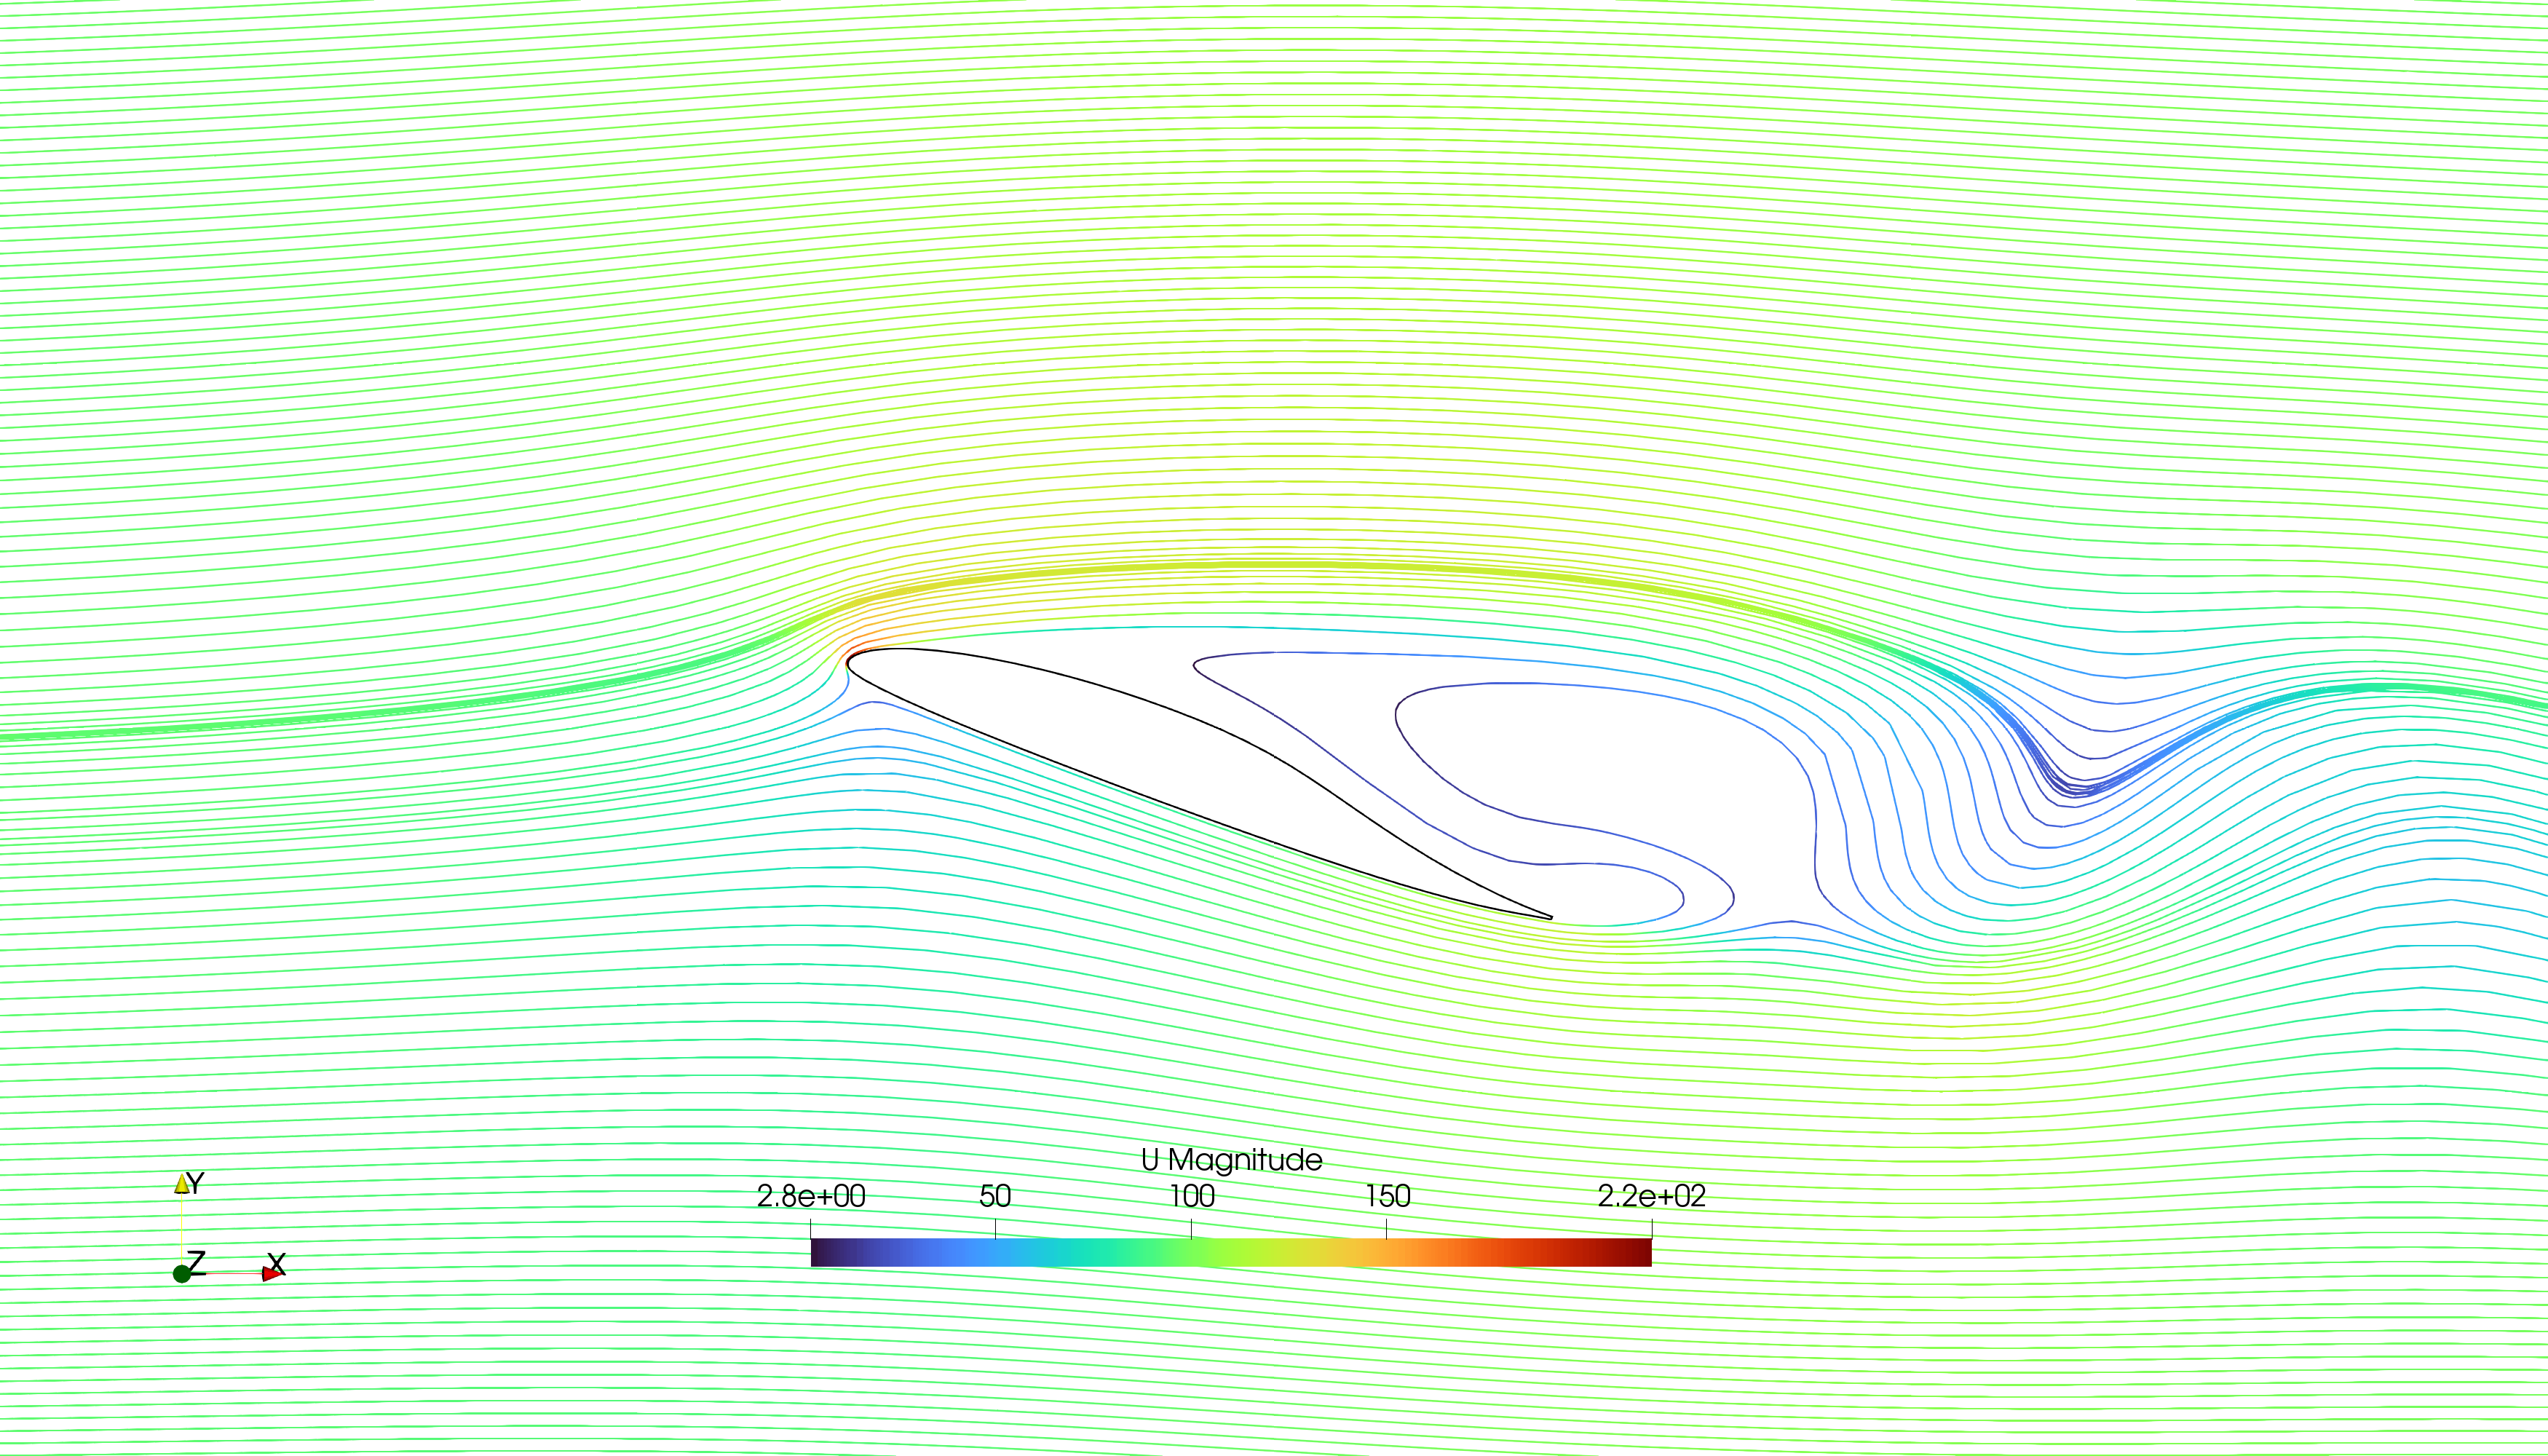
\includegraphics[width=\linewidth]{../CFD/Streamlines/20deg.png}
    \caption{CFD, $\alpha=20^\circ$.}
  \end{subfigure}
  \caption{Linhas de corrente previstas pelo método dos painéis (esquerda) e
  pela simulação CFD (direita) para $\alpha = 0^\circ$, $5^\circ$ e $20^\circ$,
  de cima para baixo.}
  \label{fig:linhas}
\end{figure}

\rasc{A $0^\circ$ e a $5^\circ$ os dois métodos dão escoamentos muito
semelhantes. O escoamento mantém-se colado em todo o perfil, o ponto de
estagnação fica junto ao bordo de ataque (nos painéis, em $x/c \approx 0{,}002$
a $0^\circ$ e $x/c \approx 0{,}005$ no intradorso a $5^\circ$), as linhas de
corrente aproximam-se no extradorso, onde o escoamento acelera, e saem
suavemente pelo bordo de fuga. No método dos painéis esta saída é imposta pela
condição de Kutta, enquanto no CFD resulta naturalmente da viscosidade.

A $20^\circ$ os dois resultados são completamente diferentes. No método dos
painéis o escoamento continua colado, com o ponto de estagnação no intradorso
($x/c \approx 0{,}105$) e o escoamento a contornar o bordo de ataque com uma
aceleração muito elevada ($C_{p,\min} \approx -21{,}8$). Isto não acontece na
realidade, porque um gradiente adverso de pressão desta ordem faria descolar a
camada limite. É isso que se vê no CFD, onde a camada limite descola junto ao
bordo de ataque e se forma uma grande zona de recirculação sobre todo o
extradorso, com uma esteira larga, o que explica a
queda de $c_l$ e o aumento de $c_d$.}

\paragraph{Coeficiente de pressão.}
A Figura~\ref{fig:cp} compara as distribuições de $C_p$ previstas pelos dois
métodos, e a Tabela~\ref{tab:estagnacao} apresenta a posição do ponto de
estagnação e o $C_p$ mínimo.

\begin{figure}[H]
  \centering
  \placeholder[0.32\linewidth]{4cm}{$C_p$, $0^\circ$\\painéis + CFD}\hfill
  \placeholder[0.32\linewidth]{4cm}{$C_p$, $5^\circ$\\painéis + CFD}\hfill
  \placeholder[0.32\linewidth]{4cm}{$C_p$, $20^\circ$\\painéis + CFD}
  \caption{Coeficiente de pressão ao longo do perfil previsto pelo método dos
  painéis e pela simulação CFD para $\alpha = 0^\circ$, $5^\circ$ e $20^\circ$.}
  \label{fig:cp}
\end{figure}

\begin{table}[H]
  \centering
  \caption{Posição do ponto de estagnação e coeficiente de pressão mínimo.}
  \label{tab:estagnacao}
  \begin{tabular}{ccccc}
    \toprule
    & \multicolumn{2}{c}{Ponto de estagnação, $x/c$} & \multicolumn{2}{c}{$C_{p,\min}$ ($x/c$)} \\
    $\alpha$ & Painéis & CFD & Painéis & CFD \\
    \midrule
    $0^\circ$  & \rasc{0,002} & \tbd{} & \rasc{$-0{,}56$ (0,007)} & \tbd{} \\
    $5^\circ$  & \rasc{0,005} & \tbd{} & \rasc{$-1{,}16$ (0,024)} & \tbd{} \\
    $20^\circ$ & \rasc{0,105} & \tbd{} & \rasc{$-21{,}8$ (0,001)} & \tbd{} \\
    \bottomrule
  \end{tabular}
\end{table}

\tbd{Análise: deslocamento do ponto de estagnação para o intradorso
com $\alpha$; pico de sucção maior nos painéis; patamar de $C_p$ no CFD a
$20^\circ$ (escoamento descolado).}

\paragraph{Gama linear.}
Como os métodos potenciais são lineares por construção, a gama linear do perfil
identifica-se pelo CFD. \rasc{Os incrementos de $c_l$ no CFD, por cada
$5^\circ$, são de $0{,}57$, $0{,}52$, $0{,}18$ e $-0{,}29$. Entre $5^\circ$ e
$10^\circ$ o declive é 9\,\% inferior ao inicial, ainda dentro da tolerância,
mas entre $10^\circ$ e $15^\circ$ cai para cerca de um terço, e a partir daí
$c_l$ diminui. A gama linear vai, portanto, de $0^\circ$ a $\approx 10^\circ$, e $c_{l,\max} \geq 1{,}34$ ocorre entre $10^\circ$ e
$20^\circ$ (a resolução de $5^\circ$ não permite localizá-lo melhor). Em cruzeiro,
$c_l \approx 0{,}22$, o que corresponde a $\alpha \approx 1{,}3^\circ$ (CFD) a
$1{,}9^\circ$ (perfis delgados), pelo que o ponto de funcionamento fica bem dentro da zona
linear, onde os três métodos diferem no máximo cerca de $0{,}06$ em $c_l$.}
% Movido da Introdução — ponto de funcionamento em cruzeiro:
% c_l = W / (1/2 rho V^2 S) = 1633*9,81 / (0,5*1,225*94,4^2*13,46) ≈ 0,22
% Comparar com a zona linear: a que alpha corresponde em cada método?

\section*{Conclusões}

\rasc{No método dos painéis, $N = 260$ painéis bastam para o $c_l$ a $5^\circ$
ficar a menos de 0,5\,\% do valor obtido com 800 painéis. No CFD escolheu-se a
malha com cerca de 64 mil células, para a qual a incerteza relativa do $c_l$
entre malhas é de 1,3\,\%.

Os três métodos dão um ângulo de sustentação nula pequeno e negativo, entre
$-0{,}67^\circ$ e $-0{,}13^\circ$, porque a subida da linha média junto ao bordo
de fuga anula quase todo o efeito da curvatura.

Na zona linear, o método dos painéis prevê o maior declive (6,78~rad$^{-1}$)
por incluir a espessura. O CFD (6,26~rad$^{-1}$) fica praticamente igual à
teoria dos perfis delgados ($2\pi$), porque o aumento devido à espessura é
compensado pela redução devida à viscosidade.

O CFD é linear até cerca de $10^\circ$ e o perfil entra em perda entre $15^\circ$
e $20^\circ$. A $20^\circ$ o escoamento está descolado em quase todo o
extradorso e não é estacionário, o que os métodos potenciais, que admitem
escoamento sempre colado, não conseguem prever.

A $0^\circ$ e a $5^\circ$ as linhas de corrente e as distribuições de $C_p$ dos
painéis e do CFD são muito parecidas. A $20^\circ$ os painéis preveem um pico de
sucção de $-21{,}8$, enquanto o CFD mostra um pico muito menor e um patamar de
pressão no extradorso, típico do escoamento descolado.

Os métodos potenciais calculam toda a curva $c_l(\alpha)$ em pouco mais de um
segundo e chegam para estimar $c_l$ e $\alpha_{L=0}$ na zona linear. O CFD
demora minutos por ângulo e exige muito mais preparação, mas é o único que
serve perto e depois da perda e para obter o arrasto.

\paragraph{Uso de inteligência artificial.} Utilizou-se IA (Claude, da
Anthropic) como apoio na programação em MATLAB (painelização, geração de figuras
e correção de código), na formatação do relatório em \LaTeX{} e na redação de
rascunhos do texto, que foram revistos pelo grupo.}
\tbd{confirmar com o grupo onde foi usada}

% Referências por ordem de primeira citação no texto.
\begin{thebibliography}{99}

\bibitem{wiki_sr20}
Wikipedia, ``Cirrus SR20''. Disponível em:
\url{https://en.wikipedia.org/wiki/Cirrus_SR20} (consultado a 25/11/2026).

\bibitem{afm_nortavia}
AFM.aero, ``Portuguese Flight School Nortavia Highlights Role as Certified Cirrus
Training and Service Hub'', 18/01/2026. Disponível em:
\url{https://afm.aero/portuguese-flight-school-nortavia-highlights-role-as-certified-cirrus-training-and-service-hub}.

\bibitem{uiuc}
UIUC Applied Aerodynamics Group, \emph{UIUC Airfoil Data Site}: D.~Lednicer,
\emph{The Incomplete Guide to Airfoil Usage}, e M.~S.~Selig, \emph{UIUC Airfoil
Coordinates Database} (ficheiro \texttt{marske7.dat}). Disponível em:
\url{https://m-selig.ae.illinois.edu/ads.html} (consultado a 25/11/2026).

\bibitem{blueprint_sr22}
The-Blueprints.com, ``Cirrus SR22''. Disponível em:
\url{https://the-blueprints.com/blueprints/modernplanes/modern-c/80996/view/cirrus_sr22}
(consultado a 25/11/2026).

\bibitem{easa_tcds}
European Union Aviation Safety Agency, \emph{Type-Certificate Data Sheet
EASA.IM.A.007 -- SR20, SR22, SR22T}, Issue~19, 22/04/2026. Disponível em:
\url{https://www.easa.europa.eu/en/downloads/7512/en}.

\bibitem{airplaneslist}
Universidade de Aveiro, 43947 Aerodinâmica, \emph{Reference list of airplanes},
2026/2027.

\bibitem{anderson}
J.~D.~Anderson, Jr. e C.~P.~Cadou, \emph{Fundamentals of Aerodynamics}, 7.ª ed.
Nova Iorque, NY, EUA: McGraw-Hill, 2024.

\bibitem{katz}
J.~Katz e A.~Plotkin, \emph{Low-Speed Aerodynamics}, 2.ª ed. Cambridge, Reino
Unido: Cambridge University Press, 2001. DOI: 10.1017/CBO9780511810329.

\bibitem{openfoam}
The OpenFOAM Foundation, \emph{OpenFOAM User Guide}. Disponível em:
\url{https://doc.cfd.direct/openfoam/user-guide} (consultado a 25/11/2026).

\bibitem{mesh_independence}
I.~B.~Celik, U.~Ghia, P.~J.~Roache, C.~J.~Freitas, H.~Coleman e P.~E.~Raad,
``Procedure for estimation and reporting of uncertainty due to discretization
in CFD applications'', \emph{Journal of Fluids Engineering}, vol.~130,
n.º~7, artigo 078001, 2008. DOI: 10.1115/1.2960953.

\end{thebibliography}

\end{document}
